\documentclass{mproj}
\usepackage{graphicx}

\usepackage{url}
\usepackage{fancyvrb}
\usepackage[final]{pdfpages}
\usepackage{times}
\usepackage{listings}
\usepackage{xcolor}
\usepackage{booktabs, multirow}
\usepackage{soul}
\usepackage{changepage,threeparttable}
\usepackage{amsmath}
\usepackage{enumitem}
\usepackage{mathtools}
\usepackage{tabularx}

% \usepackage[demo]{graphicx}
\usepackage{caption}
\usepackage{subcaption}

\lstset {
    language=C++,
    backgroundcolor=\color{black!5},
    basicstyle=\footnotesize,
    numbers=left,
    stepnumber=1,
    showstringspaces=false,
    tabsize=1,
    breaklines=true,
    breakatwhitespace=false,
}

\setlist{nolistsep}

% for alternative page numbering use the following package
% and see documentation for commands
%\usepackage{fancyheadings}


% other potentially useful packages
%\uspackage{amssymb,amsmath}
%\usepackage{url}
%\usepackage{fancyvrb}
%\usepackage[final]{pdfpages}

\begin{document}

%%%%%%%%%%%%%%%%%%%%%%%%%%%%%%%%%%%%%%%%%%%%%%%%%%%%%%%%%%%%%%%%%%%
\title{Social Distancing Detector with Deep Learning and Parallel Computing on Android Application}
\author{Jinkawin Phongpawarit}
\date{21 September 2020}
\maketitle
%%%%%%%%%%%%%%%%%%%%%%%%%%%%%%%%%%%%%%%%%%%%%%%%%%%%%%%%%%%%%%%%%%%

%%%%%%%%%%%%%%%%%%%%%%%%%%%%%%%%%%%%%%%%%%%%%%%%%%%%%%%%%%%%%%%%%%%
\begin{abstract}
    Due to pandemic on this year, social distancing has been recommended
    by the government, and this can reduce the spread of disease.
    With the help of technology, social distancing violation can be determined by using computational devices, such as mobile phone.
    To determine social distancing violation, firstly,
    humans are detected by using deep neural network.
    Then, the distance will be calculated among detected humans.
    This dissertation is developing social distancing detection on Android application with the purpose of
    performance maximisation by using all tools and techniques.
    Parallel computing and NEON instruction are used for performance enhancement.
    To detect humans by using deep neural network, OpenCV, a third-party library, is used in this project.
    OpenCV is used for network initialisation, and forwarding preprocessed input through the network.
    To understand performance maximisation,
    there are comparisons among detection models, technologies, and programming languages.
    Comparisons and evaluation of the performance are presented in this dissertation.
    The results show that parallel computing and NEON instruction improve the application's performance.
    In addition, the performance is better when OpenCV is manually built.
    Moreover, the performance is improved with speed-up up to 52 per cent.
\end{abstract}

%%%%%%%%%%%%%%%%%%%%%%%%%%%%%%%%%%%%%%%%%%%%%%%%%%%%%%%%%%%%%%%%%%%

%%%%%%%%%%%%%%%%%%%%%%%%%%%%%%%%%%%%%%%%%%%%%%%%%%%%%%%%%%%%%%%%%%%
\educationalconsent

%%%%%%%%%%%%%%%%%%%%%%%%%%%%%%%%%%%%%%%%%%%%%%%%%%%%%%%%%%%%%%%%%%%

\newpage
%%%%%%%%%%%%%%%%%%%%%%%%%%%%%%%%%%%%%%%%%%%%%%%%%%%%%%%%%%%%%%%%%%%
\section*{Acknowledgements}
    I would like to express my very great appreciation to my supervisor,
    Dr Jose Cano Reyes, for his mentorship throughout the whole duration of this project.
    This dissertation would not be completed without the guidance of my supervisor.
    He always provided me with very invaluable advice,
    and he couraged me when I struggled in trouble;
    these have been very much appreciated.

    I would like to thank my family for their love and the opportunity of studying a master degree that I have given for a whole year. It is the most valuable experience of my life.
    Last but not least, I would like to thank my friends who have supported and encouraged me during
    the past year.

%%%%%%%%%%%%%%%%%%%%%%%%%%%%%%%%%%%%%%%%%%%%%%%%%%%%%%%%%%%%%%%%%%%
\tableofcontents
%%%%%%%%%%%%%%%%%%%%%%%%%%%%%%%%%%%%%%%%%%%%%%%%%%%%%%%%%%%%%%%%%%%

%%%%%%%%%%%%%%%%%%%%%%%%%%%%%%%%%%%%%%%%%%%%%%%%%%%%%%%%%%%%%%%%%%%
\chapter{Introduction}\label{intro}
    \section{Motivation}

        % - Introduction
            There are pandemics over hundreds years, including flu pandemic in 1918 and the black death in 1346 ~\cite{REF1-01}, ~\cite{REF1-02}.
            There were millions people died during each pandemic.
            This year, humanity is facing the other pandemic, which is named as coronavirus or COVID-19.
            However, COVID-19 can be well-managed with scientific discovery and technology.
            For instance, social distancing has been recommended since there was Influenza A (H1N1) pandemic in 2009 ~\cite{REF1-05}.
            It is able to reduce the spread, and slow down and reduce the size of the epidemic peak ~\cite{REF1-03}, ~\cite{REF1-04}.
            Consequently, an infection curve is flattened, and the number of deaths is reduced.
            Yet, scientific researchers still work continuously on this outbreak.
            In addition, technology can be integrated with scientific theory to gain advantages.

        % - Problem statement


        -	Why I choose mobile application \\
            - Mobile become popular device which people use for everything (such as receiving news, study or business purpose) \\
            - 1. Performance \\
                - One technology that has high competition -> high improvement is mobile \\
                - Since the first smartphone, it has been evolved a lot \\
                - It increases capability of phone (CPU, GPU, and Memory) which is able to perform many tasks as desktop computer \\
            - 2. Portability \\
                - No charger is needed during being used \\
                - Mobile have all needed function (camera, computation hardware - CPU) \\
                - Move computation part from server to device \\
            - 3. Can be enhance by parallel computing \\

    \section{Objectives}
        -	Android application is able to do social distancing detection by using Deep Neural Network (DNN) \\
        -	Able to do the task in parallel \\
        -	Use camera to detect in the real-time \\
        -   Use all techinique and technology to improve the perfoormance \\

    \section{Structure}
        The content of this dissertation is structured as follows: \\
        1.	Chapter 2 provides a background knowlegde of Android application, object detection, distance calculation, and parallel computing. \\
        2.	Chapter 3 shows an overview of the system, class diagram, and design.  \\
        3.	Chapter 4 describes implementation details and technical development. \\
        4.	Chapter 5 analyses development's problems and the performance evaluation. \\
        5.	Chapter 6 concludes results of the project, limitation, and future works.  \\


%%%%%%%%%%%%%%%%%%%%%%%%%%%%%%%%%%%%%%%%%%%%%%%%%%%%%%%%%%%%%%%%%%%
\chapter{Background and Related Works}\label{background}

    This chapter aims to introduce background knowledge that relates to this project including deep neural network, android development, and distance calculation.
    Then, this chapter gives examples of related works.

    \section{Deep Neural Network}
        A Deep Neural Network (DNNs) is a deep learning's architecture,
        which is a part of machine learning, and it is based on artificial intelligence.
        DNN is stimulated from the human nervous system, which contains cells.
        These cells are called neurons, and they are fully linked \cite{deep-learing-2}.
        Likewise, DNNs are composed of multiple layers between input and output,
        and each layer has neurons, which are entirely connected \cite{deep-learing-3}.
        These layers turn input to output by passing data through each layer and doing some computation,
        and this is called forward propagation \cite{deep-learing-2}, \cite{deep-learing-1}.
        DNN can be applied in many fields such as computer vision (CV), speech recognition, or object detection \cite{deep-learing-1}.


    \section{Threading in Android}
        Threads in Android development are split into two main categories: the main thread and a worker thread.
        A main thread or UI thread is a thread that dispatch events of user interface widgets.
        The events are dispatched regarding Android's activity lifecycle,
        and all events are managed by only one thread.
        In other words, threads will not be spawned for handling a single event or component.
        Thus, if there is a long-running task, which is run by UI thread, events cannot be delivered
        because long-running task block UI thread.
        If UI thread is blocked more than 5 seconds,
        an application will show "Application not Responding"  \cite{ANDROID-01}.

        \begin{figure}[!ht]
            \centering
            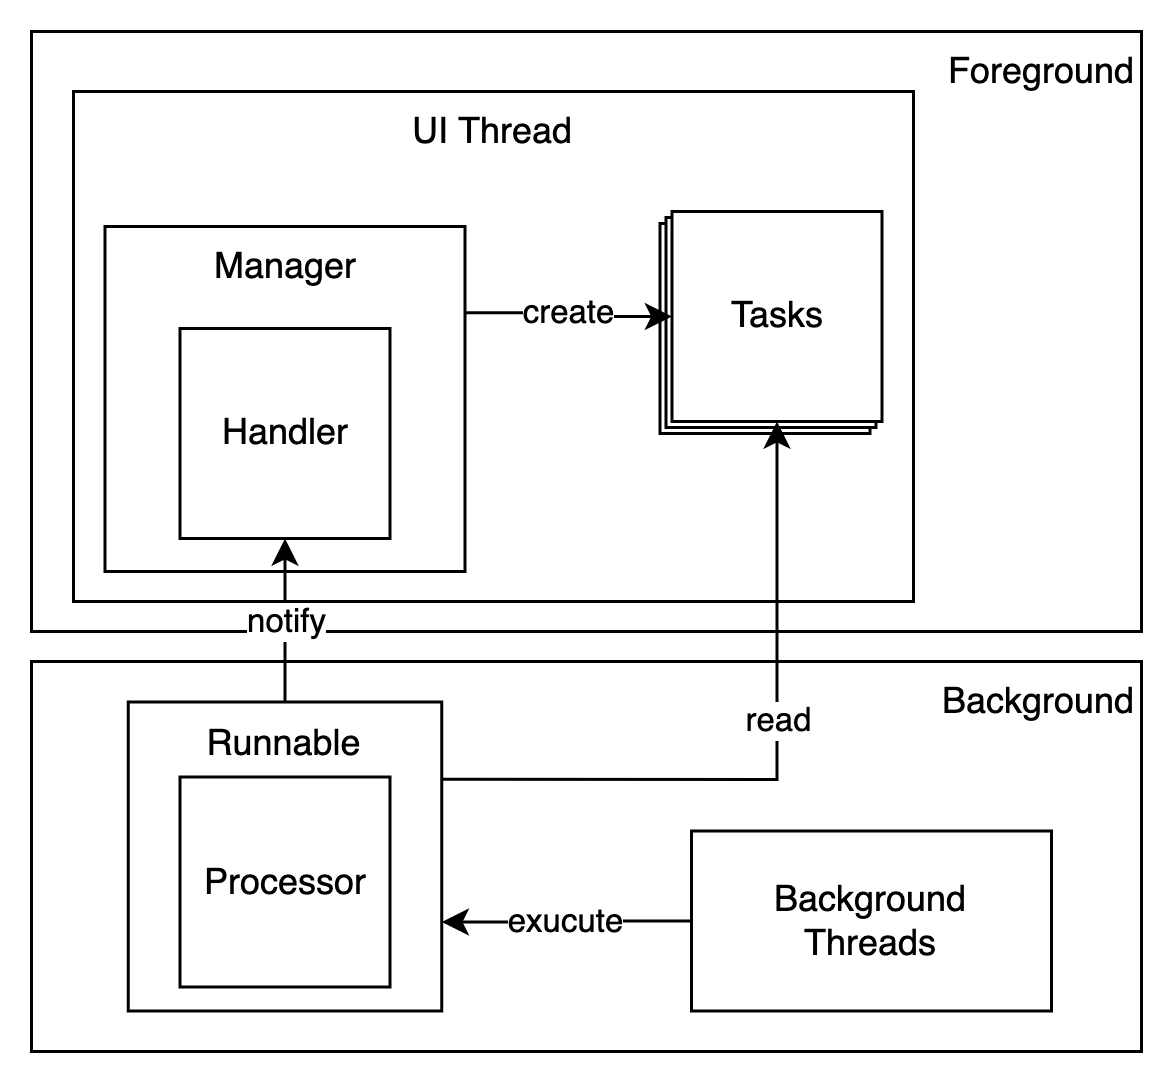
\includegraphics[width=3in]{images/chapter2/thread-overview.png}
            \caption{Threading Overview}
            \label{thread-overview}
        \end{figure}

        A working thread is separated from the UI thread to avoid freezing application,
            and it is called worker thread or background thread.
            This thread is able to process a long-running task in the background without interrupting the UI thread.
        In addition, the priority of the thread can be set from -20 to 19---the lowest priority is 19 and the highest priority is -20.
            The default value of background threads priority is 10,
            and the default value of foreground threads is -2 \cite{ANDROID-02}.

        UI thread and background thread run on different threads,
        thus a Handler is needed when there is communication between these threads.
        For example, as shown in Figure \ref{thread-overview},
        processes are divided into two parts: foreground and background.
        Tasks are created by a manager which is running on the UI thread.
        Then, Runnable, a component that can be run by background threads, will read tasks.
        After that, Runnable will be executed by background threads.
        Finally, Runnable will notify the manager through Handler.

    \section{Distance Calculation}\label{sectionDistanceCalculation}
        According to Gurucharan \cite{SOCIAL-DISTANCING-DETECTION}, to measure a distance between 2 people, the reference points of them are used for calculation.
        The reference point is the coordination of the 2 people, which is the centre of the detection frame.
        The calculation formula is based on Euclidean distance:

        \begin{equation*}
            d = \sqrt{(a_{0}-b_{0})^{2}+(D/c)\times(a_{1}-b_{1})^{2}}
        \end{equation*}

        \begin{equation*}
            c = \frac{a_{1}+b_{1}}{2}
        \end{equation*}

        However, a three-dimensional space is captured into a two-dimensional image,
        so depth and perspective can be seen in Figure \ref{distanceCalculation}.
        Thus, a couple of variables are added into the formula.
        The first variable is $D$, which is the diagonal of the image.
        The second variable is $c$, which is a calibration.
        These two variables will determine the depth of people in the image.

        \begin{figure}[h!]
            \centering
            \begin{subfigure}{.5\textwidth}
              \centering
              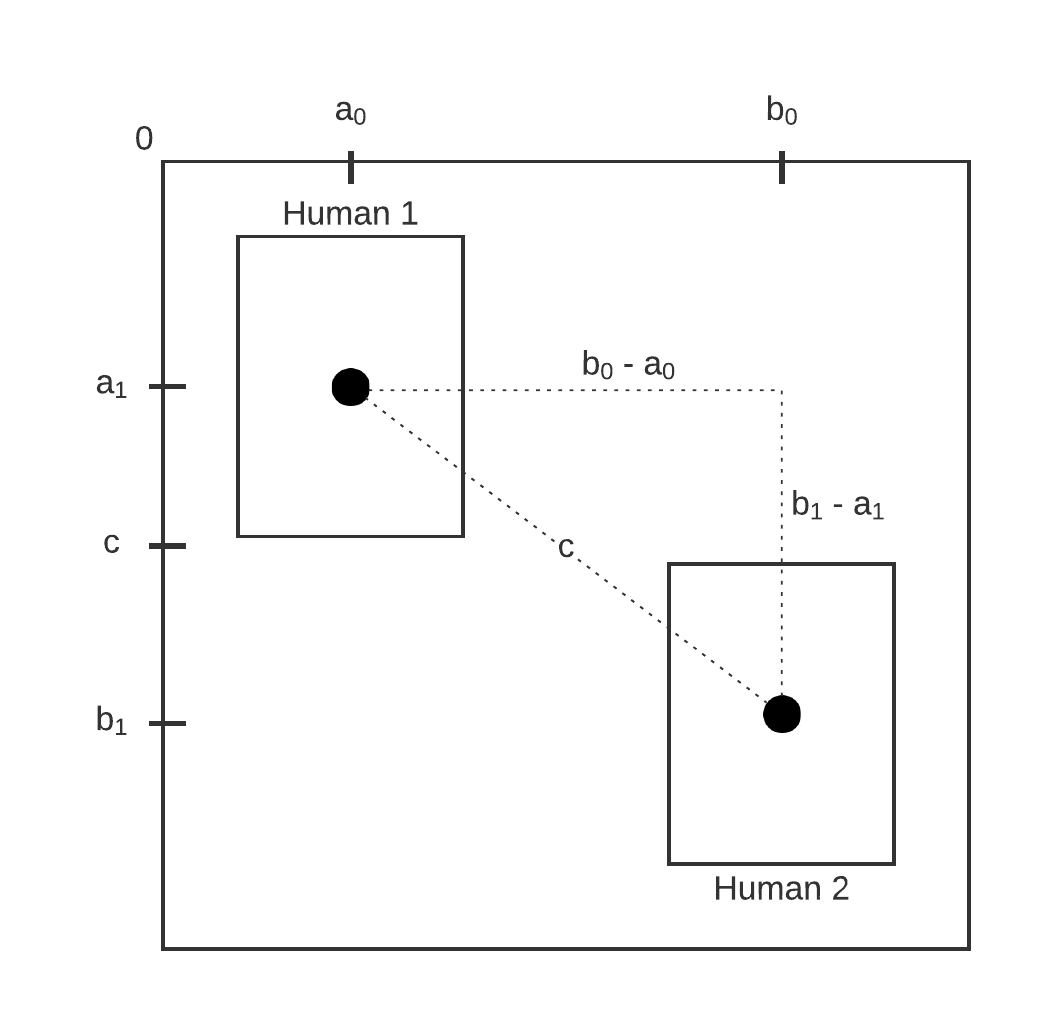
\includegraphics[width=2.5in]{images/chapter2/distance.png}
              \caption{Distance calculation}
              \label{distanceCalculation}
            \end{subfigure}%
            \begin{subfigure}{.5\textwidth}
              \centering
              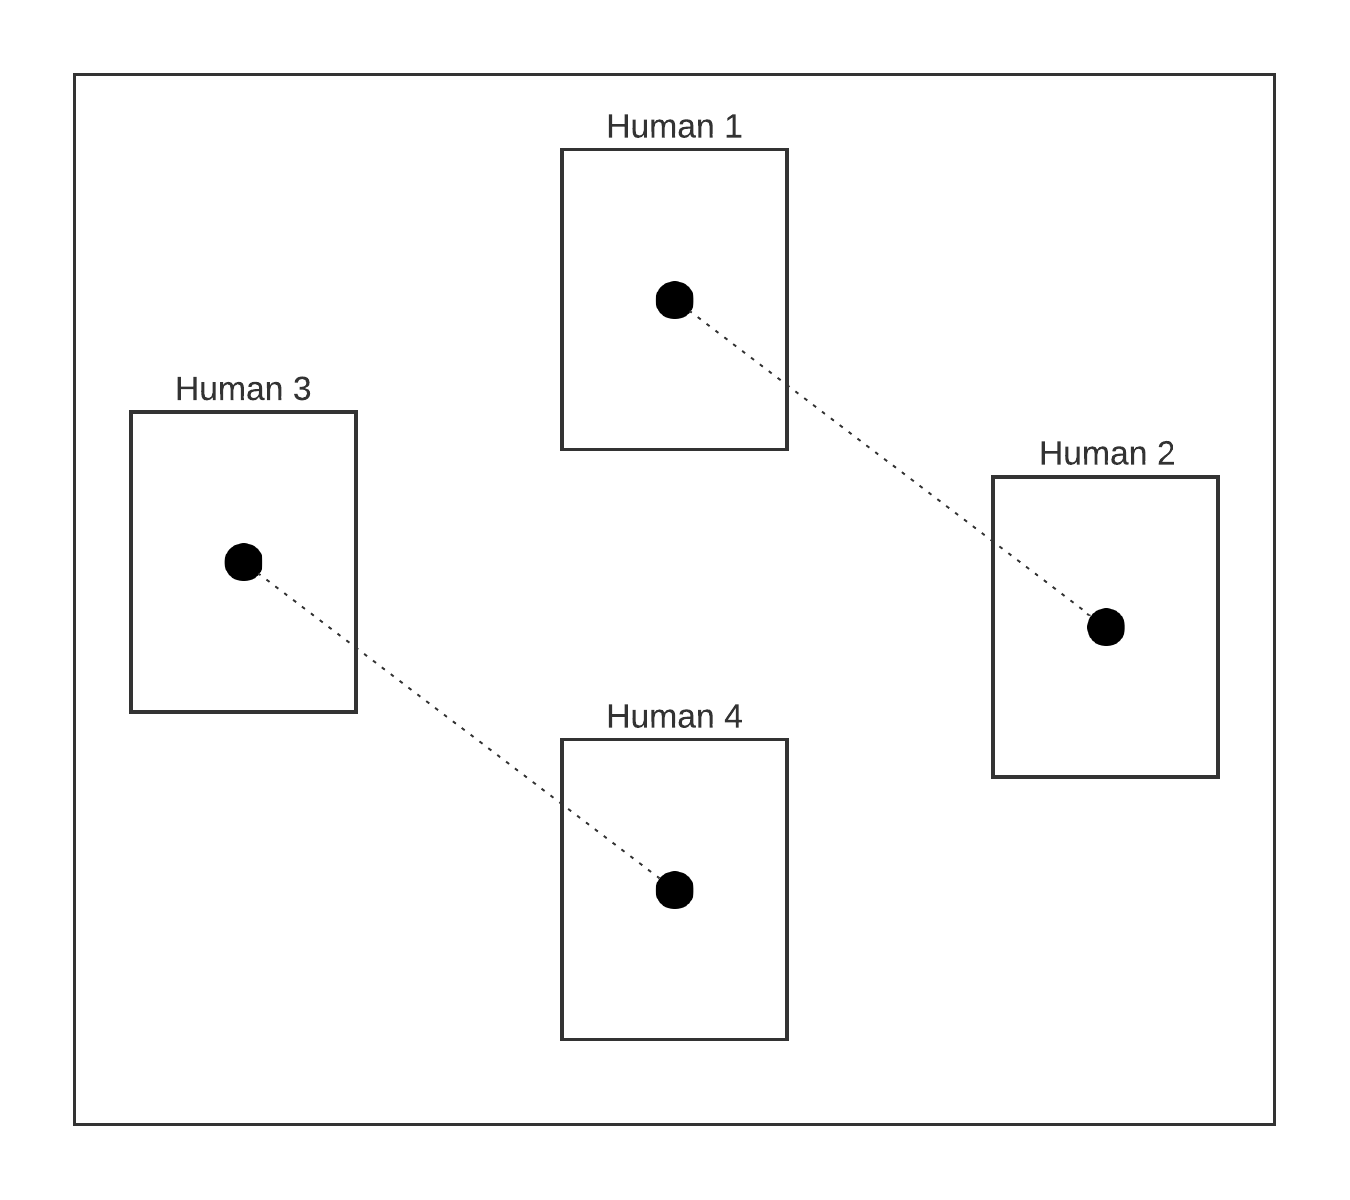
\includegraphics[width=2.5in]{images/chapter2/two-distances.png}
              \caption{A difference of 2 distances}
              \label{twoDistances}
            \end{subfigure}
            \caption{Determining Social Distancing}
            \label{determiningConcept}
        \end{figure}

        For example, according to Figure \ref{twoDistances},
        if the distance is calculated without calibration, the distance between 2 groups of people will be the same.
        Naturally, the distance between Human1 and Human2 must be further than the distance between Human3 and Human4.

    \section{Related Work}
        \subsection{Object Detector}
            Object Detector is an Android application\footnote{https://play.google.com/store/apps/details?id=com.tecomen.android.objectdetector},
            which is able to detect objects through a camera.
            This application is implemented by a deep learning library from TensorFlow \cite{tensorflow2015-whitepaper} with
            MobileNet model\footnote{https://tfhub.dev/tensorflow/lite-model/ssd\_mobilenet\_v1/1/metadata/1?lite-format=tflite} \cite{mobilenet} \cite{ssd} and COCO dataset \cite{coco-dataset}. There are two modes in this application,
            which are detection mode and classification mode.
            The processing time of each frame is 250 to 300 milliseconds.
            The screenshot of the application can be seen in Figure \ref{appendix:obj-detector}.

        \subsection{TensorFlow Object Detection}
            TensorFlow Object Detection is an object detection application\footnote{https://play.google.com/store/apps/details?id=org.tensorflow.detect},
            which is run on the Android operating system.
            TensorFlow's library is used in this application, along with the MobileNet model.
            This application is able to detect objects in real-time from the camera.
            The screenshot of the application can be seen in Figure \ref{appendix:ts-obj-detection}.


        \subsection{Computer Vision Detection}
            Computer Vision Detection application operates on the Android operating system\footnote{https://play.google.com/store/apps/details?id=com.pobeda.ivan.opencvdetect}.
            This application is able to process real-time video from a live camera,
            and OpenCV is used as a library \cite{opencv_library}.
            There are 12 options of algorithms, such as colour detector, canny detector, motion detector, and shape detector.
            Besides, this application is able to detect human faces and smiling faces.
            This application is able to process around 13 frames per second.
            The screenshot of the application can be seen in Figure \ref{appendix:cv-detection}.

        \subsection{Real Time Object Detection and Tracking Using Deep Learning and OpenCV}
            Demonstrates and explains how objects are detected and tracked in real-time \cite{related-work-1}.
            Objects are detected by using Single Shot Detector algorithm (SSD),
            which is trained with MobileNet.
            In this paper, many techniques are used to enhance the performance of the detection.
            At the first step, frames are extracted from the camera.
            Then, a local mean algorithm is applied to filter noise,
            and reduce the complexity and computing time of preprocessing.
            In addition, background subtraction is used to localise the detected object in the frame.
            The detected object is considered as a foreground object,
            and it is separated from background for further processing.
            Furthermore, the object will be tracked after the object is detected,
            which reduce the processing time because detection can be processing a few frames,
            while tracking the object can be processed faster.
            The result of this research shows that SSD can process the given image faster than YOLO model,
            and SSD can detect the object with confidence over 98\%.
            In addition, this work shows that humans can be detected with an accuracy of 99\%

%%%%%%%%%%%%%%%%%%%%%%%%%%%%%%%%%%%%%%%%%%%%%%%%%%%%%%%%%%%%%%%%%%%
\chapter{Design and Implementation}\label{implement}

    In this chapter, the implementation details will be explained in many aspects, including Java Native Interface,
    human detection, and distance calculation.

    \section{MoSCoW Statement}

        \subsection{Must have}
            \begin{itemize}
                \setlength\itemsep{1em}
                \item The application \textbf{must} be able to detect people in the given image or video.
                \item The application \textbf{must} be able to determind distancing between people in the given image or video.
                \item The application \textbf{must} save the processed image of video.
                \item The application \textbf{must} allow user to choose image or video from device's storage.
            \end{itemize}

        \subsection{Should have}
            \begin{itemize}
                \item The application \textbf{should} be able to stream video from camera.
                \item The application \textbf{should} be able to show detected people on camera.
                \item The application \textbf{should} support parallel computing.
            \end{itemize}

        \subsection{Could have}
            \begin{itemize}
                \item The application \textbf{could} choose computation options between sequencial or parallelism.
                \item The application \textbf{could} support NEON techonology.
                \item The application \textbf{could} be able to process the given tasks in background.
            \end{itemize}
        \subsection{Won't have}
            \begin{itemize}
                \item The application \textbf{won't} other objects which are not human.
                \item The application \textbf{won't} support GPU computation.
            \end{itemize}


    \section{Preparation}
        This application is implemented on the Android Operating System,
        and the target Software Development Kit (SDK) version is set at level 29, namely Android Q.
        This application is compiled and built by Android Studio version 3.5.3,
        and CMake is used for compiling C++ library with C++ version 11.
        Furthermore, OpenCV version 4.4.0, which is built as shared library, is used for image processing and object detection.
        For object detection model, there are 2 models are used: You Only Look Once and MobileNet SSD.

    \section{Java Native Interface}
        Implementation is divided into 3 layers.
            The first layer is a Java layer, which mainly interacts with a user,
            checks permissions, handles activity lifecycle, communicates with Java Native Interface (JNI), and loads native libraries.
                native libraries are compiled and built into shared libraries by a Native Development Kit (NDK).
            The second layer is JNI, which is written in C or C++.
                The task of JNI layer is being an intermediate connection between the Java layer and a C++ layer.
            The last layer is the C++ layer, which alternatively performs calculation tasks,
            including Deep Neural Network and distance calculation.

        \begin{figure}[!ht]
            \centering
            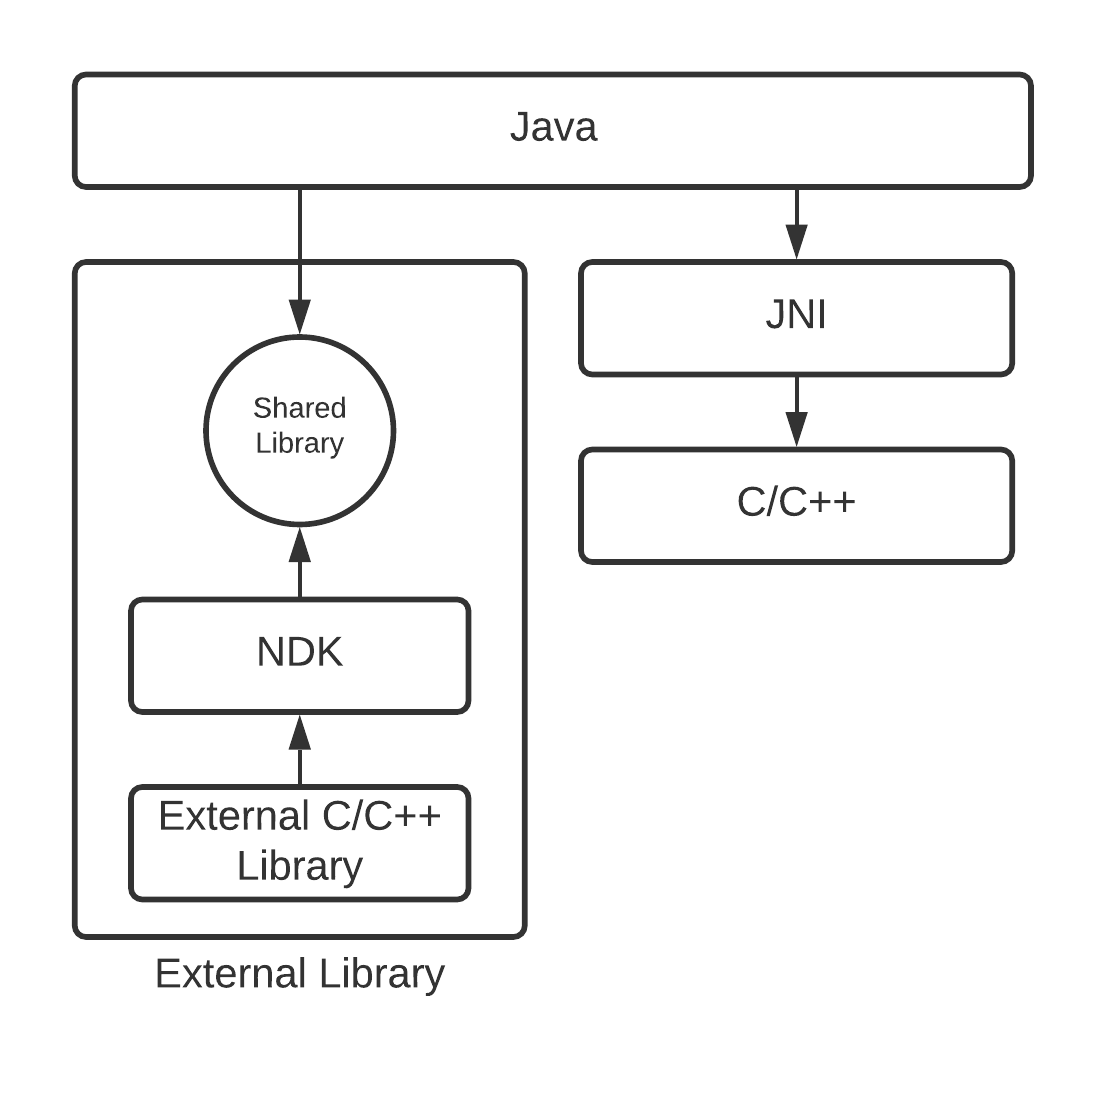
\includegraphics[width=4in]{images/chapter3/application-layers.png}
            \caption{Application Layers}
            \label{systemOverview}
        \end{figure}

        However, Deep Neural Network and distance calculation can be implemented in all layers.
        According to Android Developer Guide \cite{ANDROID-01},
        Native Development Kit (NDK) is recommended for compiling C and C++ coode into native library,
        which is able to achieve a higher performance.
        Thus, executing both tasks in the JNI and C++ layer gains a better performance.
        Furthermore, there are 2 advantages of implementing JNI.
            The first advantage is reducing JNI calling. Performing both tasks in an application layer have to call JNI methods many times,
                and this is expensive and cost an overhead.
                Thus, implementing JNI manually reduces the number of JNI calls.
            The second advantage is memory management. C++ is able to access values in the memory by using a pointer.
                Thus, values can be directly accessed without copying.

        Java and JNI communicate through native function, which is written in Java layer.
        Memory addresses of pre-processed frame in Mat format will be pass as parameter through native function,
        and it will be converted from Java type to Native type.
        Then, the given addresses will be converted back into Mat format.

\begin{lstlisting}[caption={Java Native Function},captionpos=b]
    public class NativeLib {
        static {
            System.loadLibrary("native-lib");
        }

        public native static void process(long imageAddr);
    }
\end{lstlisting}

\begin{lstlisting}[caption={C++ JNI Method},captionpos=b]
    Java_com_jinkawin_dissertation_NativeLib_process(jlong matAddr){
        Mat &frame = *(Mat *) matAddr;
        ImageProcessor::process(frame);
    }
\end{lstlisting}

    \section{Social Distancing Detection}
        % Intro to detection
        There are 3 main processes is implemented to determine social distancing violation from the image and video.

        The first process is pre-processing the given image, video, or video stram.
        The given video will be extracted into an array of images.
        Then, images will be converted into Bitmap and Mat format with RGBA colour model respectively.
        After that, colour will be converted, which depends on a detection model.
        As mentioned in section 4.1, there are 2 detection models are used for detecting humans in the given picture and video: YOLO model and MobileNet SSD model.
        Colour will be converted to RGB if the detection model is YOLO,
        while MobileNet SSD requires BGR colour model.

        \begin{figure}[!ht]
            \centering
            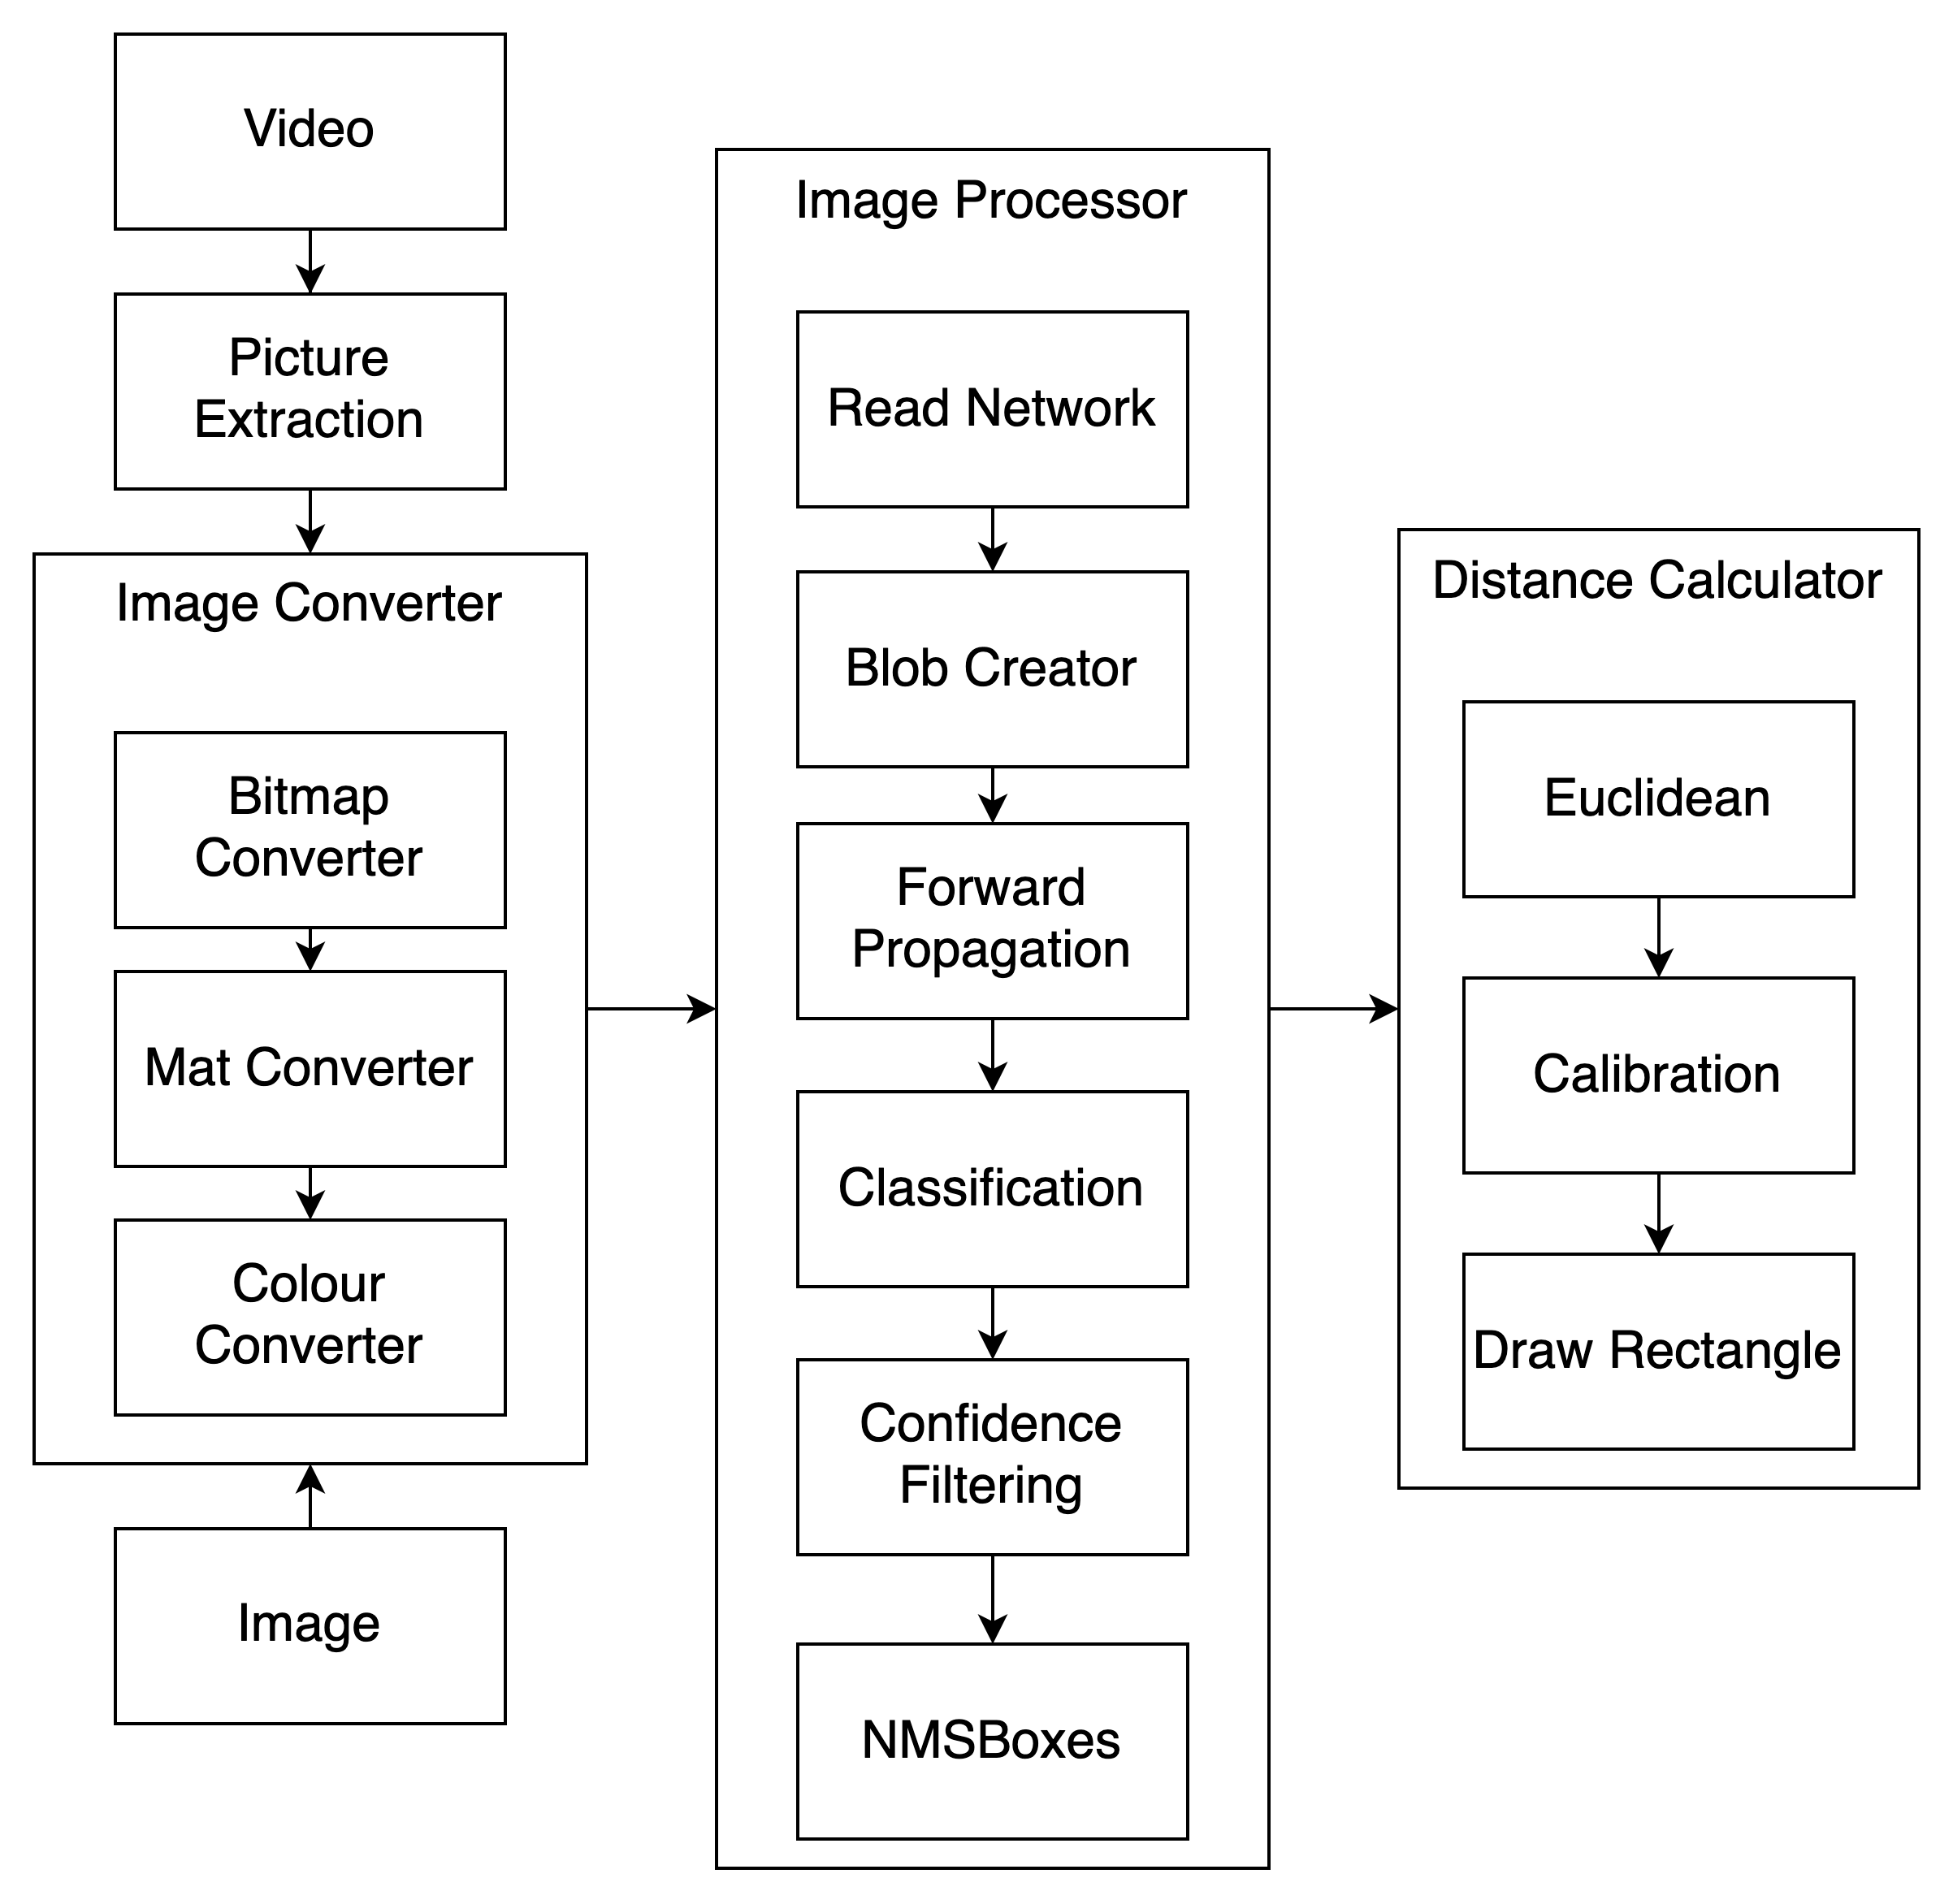
\includegraphics[width=5in]{images/chapter3/system-overview.png}
            \caption{Detection System Overview}
            \label{systemOverview}
        \end{figure}

        The second process is object detection.
        Detection models are setup and configured differently before processing images.
        First of all, YOLO is used with Darknet, which is an open source neural network framework,
            while MobileNet SSD. MobileNet is used with Caffe framework.
        Then, threshold will be set for determining the confidence score of the detected object.
            The confidence score threshold of YOLO model will be set to 0.5 or 50 percent.
            In other words, the detected object will be rejected if YOLO model cannot guarantee that a detected object is human,
            and its confidence score is lower than 50 percent.
            In contrast, the confidence score threshold of MobileNet SSD model will be set to 0.3 or 30 percent.
            Because of MobileNet SSD model has a lower ability to detect an object, the confidence threshold is set to be lower.
        After models are setup and configured, the image will be processed in 5 steps.
        For the first step, pre-processed image will be convert to input blob by passing Mat image to $blobFromImage()$ function with scale factor.
            Blob will be used for the forward propagation in the neural network.
        Secondly, blob will be passed to the network through $forward()$ function,
            and the network's output is a list of detected boxes with a label and a confidence score.
        Then, detected objects will be classified.
            Non-human objects will be removed by considering the label of the detected object.
        After that, a confidence score will be filtered by considering the threshold that is set in the configuration step.
        Finally, $NMSBoxes()$ performs non-maximum suppression, which will reduce overlapping detected boxes.

        The last process is determining social distancing.
        After a list of detected object boxes is filtered,
        the distance between each box will be calculated by using the formula which is based on Euclidean distance
        \footnote{an explanation was given in chapter \ref{background}}.
        If the value of the calculated distance is lower than the threshold,
        this mean that the couple is too close, and they are breaking social distancing rule.
        The application will change the box's colour to red.
        In contrast, if the value of the calculation is grater than threshold,
        there is no breaching of social distancing rule, and the box's colour will be changed to green.

    \section{Parallelisation}
        Multithreading is used to reduce the processing time, which can achieve nearly real-time processing.
        The strategy of multithreading is dividing an input video into frames,
        and assign frames to threads by considering a number of available cores.

        To avoid overheads, there are 2 things will be considered while application is performing mulththreading.
        Firstly, Input/Output (I/O) operation must be avoided from threading.
        Secondly, all variables should be considered due to limited memory.
            For variables, that consume a large space of heap, will be initial as static by using static block.
            In addition, the usage of short-lived variable will be reduced to avoid garbage collecting.
            Furthermore, a task will be recycled after thread finished processing the given frame.

        \begin{figure}[!ht]
            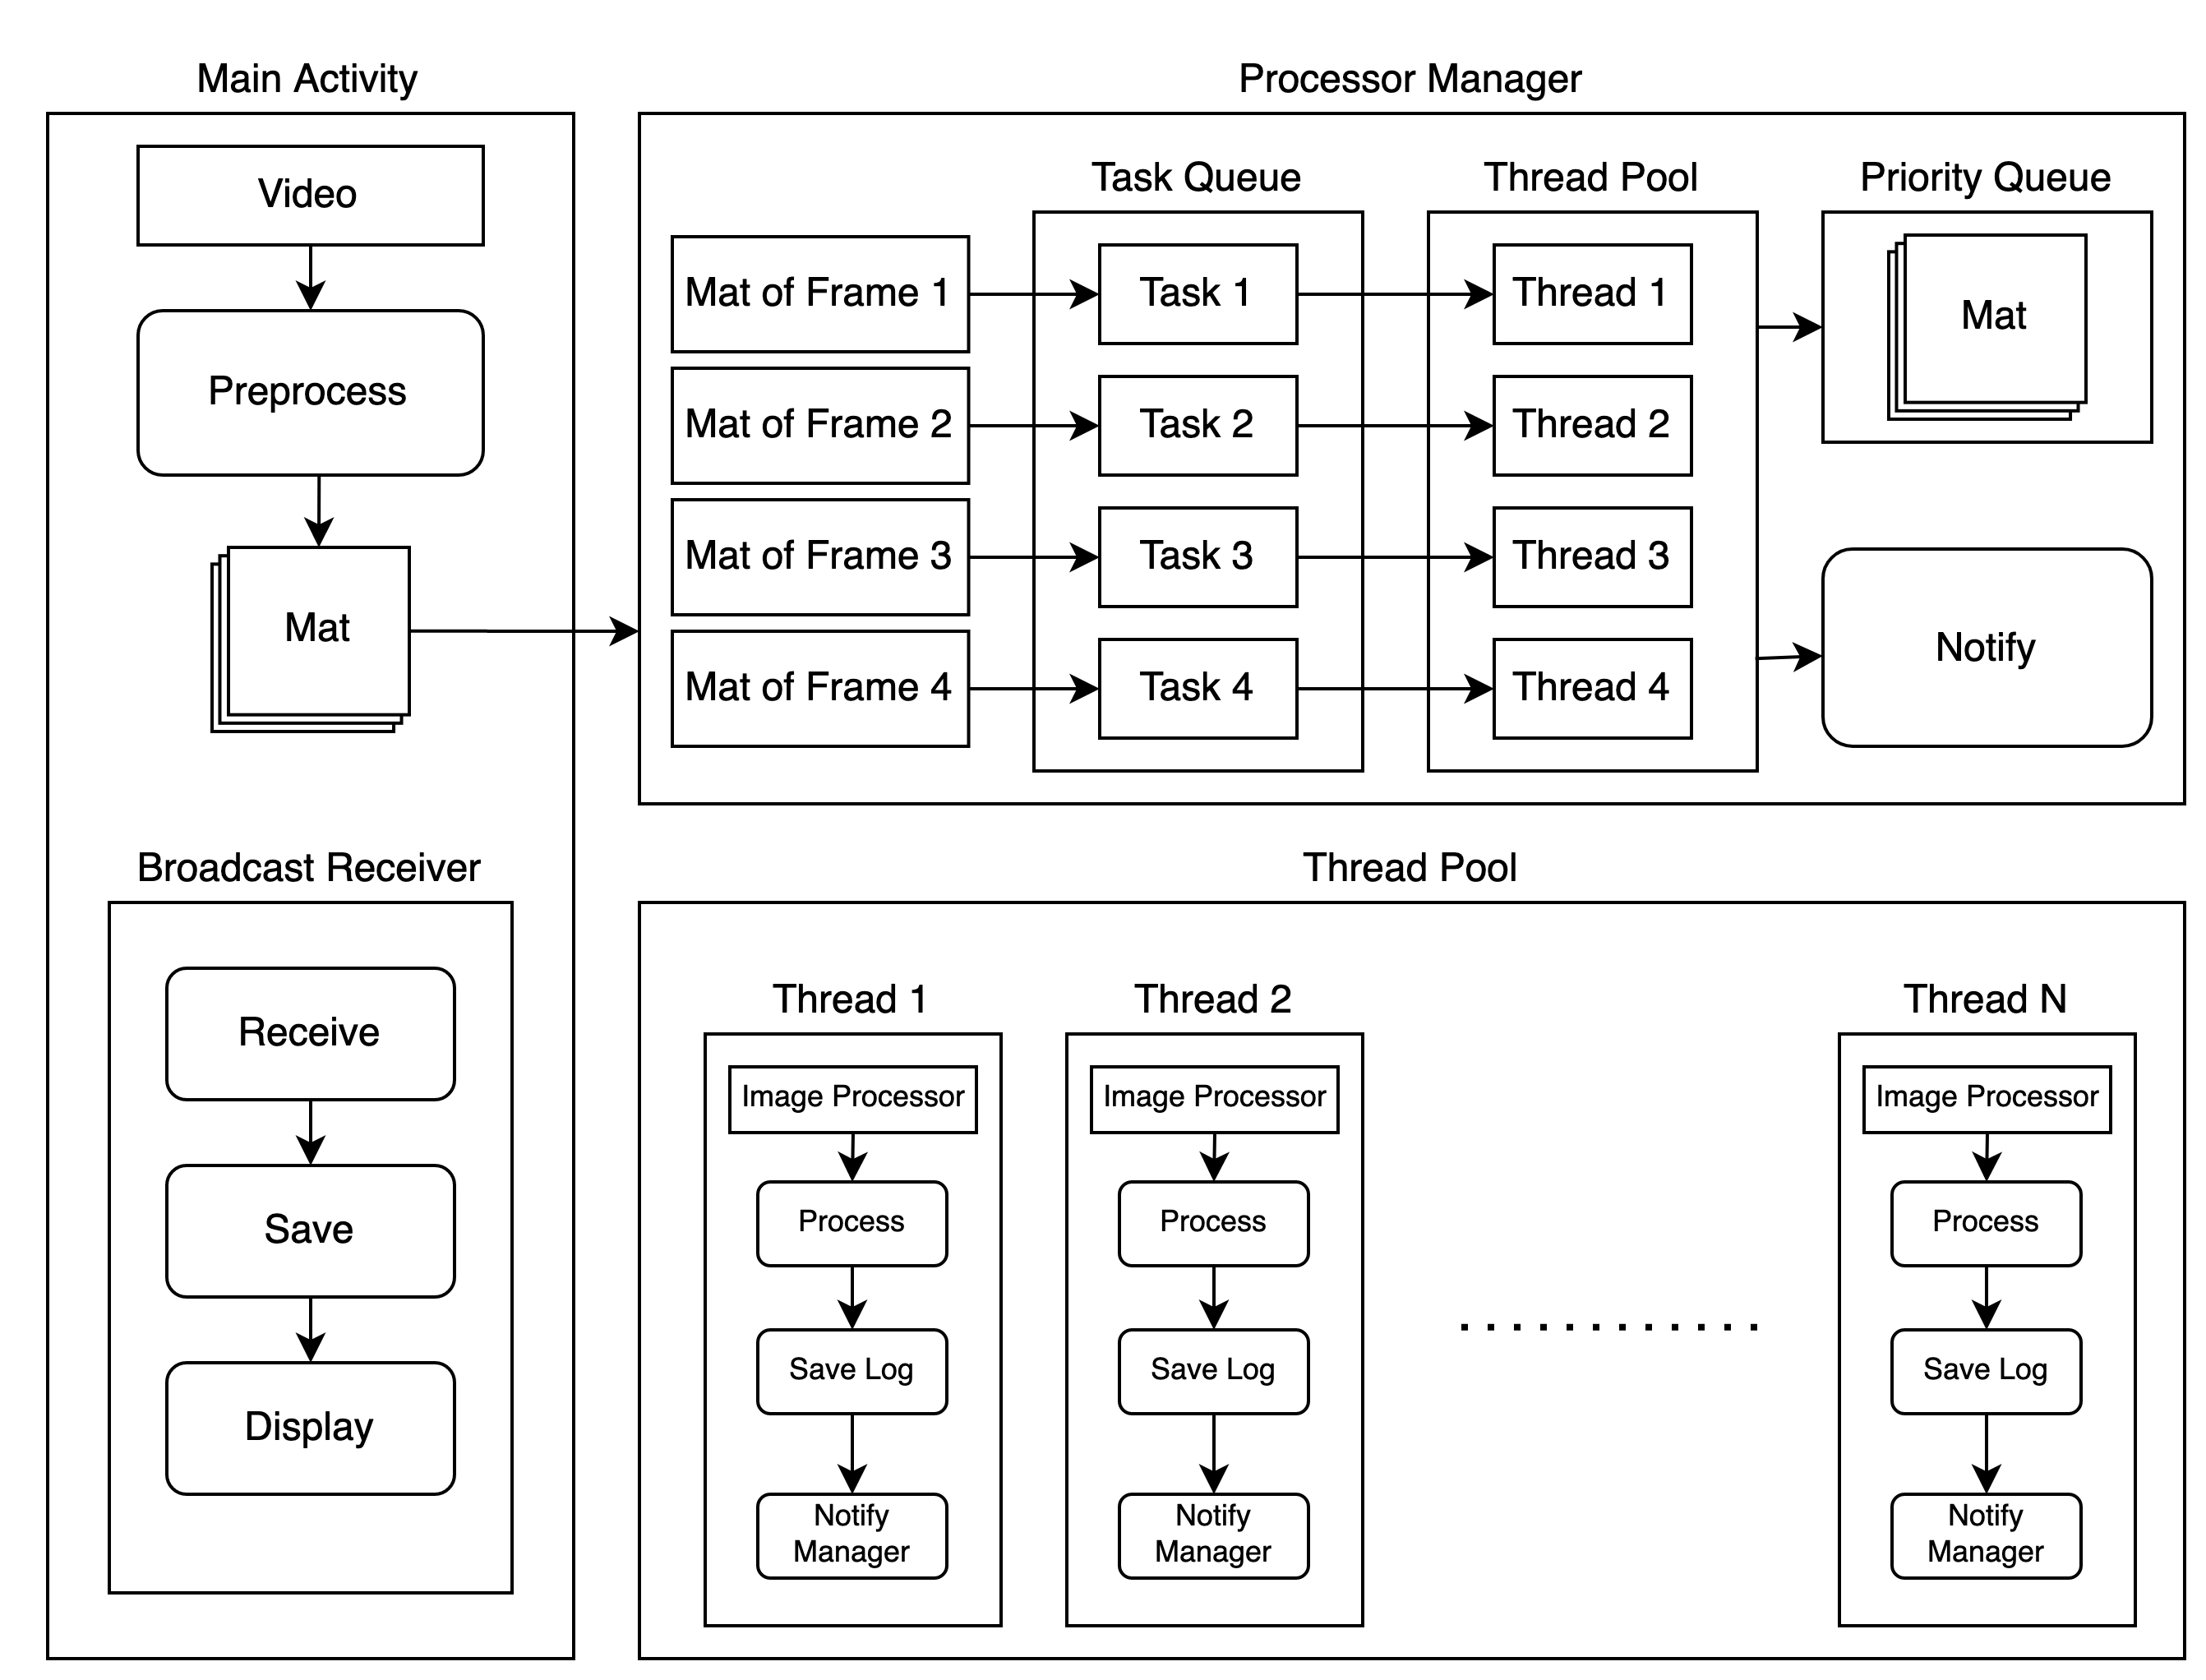
\includegraphics[width=6in]{images/chapter3/parallel.png}
            \caption{Parallel Computing Diagram}
            \label{parallelJava}
        \end{figure}

        To begin with, multithreading in Java, a processor manager is implemented for managing threads efficiently.
        To ensure that the processor manager will be created at once,
        the processor manager is designed with singleton pattern and static block.
        Thread pool and queues are fundamental operators in the processor manager.
        As can be seen in figure \ref{parallelJava}, frames in Mat format will be assigned as a task and queued in TaskQueue.
        Then, tasks will be mapped with thread orderly by the thread pool.
        A working thread will process the given task.
        After a thread finished the given task,
        the thread will write a log regarding social distancing detection, and notify the processor manager.
        Then, a task will be recyled to free up memory.
        When the processor manager receive a notification from workers,
        a processed frame will be retrieved and ordered in the priority queue.
        After the process manager retrieved all processed frames,
        the process manager will notify the main activity.
        All of these processes are run in the background to avoid a frozen application.

        On the other hand, multithreading in C++ is slightly diffent.
        The main concept of multithreading is the same as Java except thread management.
        Thread pool is implemented in Java to manage and handle threads,
        while parallelism framework in OpenCV is used in C++.
        This framework is compiled with Threading Building Blocks (TBB), which is developed by Intel.

        \begin{figure}[!ht]
            \centering
            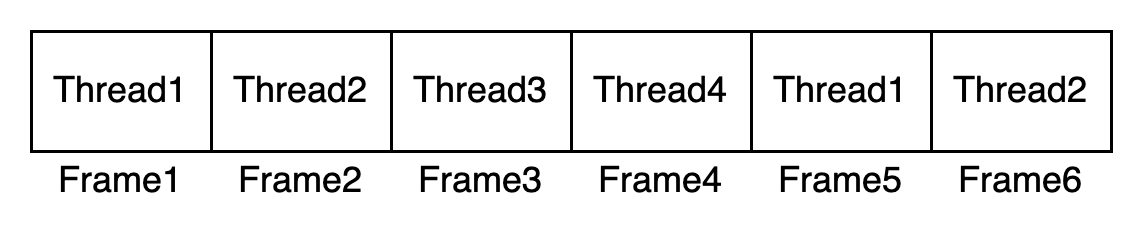
\includegraphics[width=5in]{images/chapter3/cpp-parallel.png}
            \caption{Multithreading in C++}
            \label{parallelCpp}
        \end{figure}

\begin{lstlisting}
    virtual void operator()(const cv::Range& range) const{
        for (size_t i = range.start; i < size; i += threadNo){
            cv::Mat &frame = *(cv::Mat *) frames[i];
            ImageProcessor::process(frame);
        }
    }
\end{lstlisting}

        To reduce the processing time,
        the threads will process the frame which has the same index as itself,
        and index will be incrase by the number of total available cores.
        For example, as can be seen from the figure \ref{parallelCpp},
        the first thread will process the first frame and the fifth frame.
        Theoretically, if the frame rate of video is 30 FPS and there are 4 threads,
        the first thread will have 100 miliseconds to finish processing the first frame before moving to the fifth frame.

    \section{Frame Rendering}
        The maximum processing frame rate of this application is 10 FPS, which will be discuss in chapter \ref{testing}
        At this frame rate, video cannot be displayed smoothly in live camera;
        thus, there is an algorithm that helps video can be displayed in higher frame rate.

        First of all, when a frame is streamed from the camera,
        frame will be considered to be processed or not be processed.
        Processing will be determinded from the capability of the device.
        In other words, maximum processing frame rate will be used as threadshold.
        If a number of processed frames in 1 second exceeds threadshold,
        frame will not be sent to processor manager.
        After that, the main activity will check a processed frame in priority queue from processer manager.
        If there is a processed frame in priority queue, the processed frame will be displayed to the screen.
        Otherwise, the main activity will read the last log of the processed frame, and retrieve all detection regtangles.
        Then, the main activity will draw those regtangle on the incoming frame and display it on the screen.


%%%%%%%%%%%%%%%%%%%%%%%%%%%%%%%%%%%%%%%%%%%%%%%%%%%%%%%%%%%%%%%%%%%
\chapter{Evaluation and Testing}\label{testing}

    This chapter presents an evaluation of the application, which is divided into three parts.
    The first part will show variables that must be controlled for the reliability and stability of the result.
    The second part is going to evaluate the application's performance,
    which are comparisons among models, programming languages, and technologies.
    The last section is going to show a usability testing of this application.

    \section{Controlled Variables}
        To ensure the result of the performance will not be varied by other factors, some variables must be controlled as following:
        \begin{enumerate}
            \item All testing cases will be run on Samsung Galaxy S10+.
            \item All running background applications will be closed, and memory will be freed before testing.
            \item To prevent CPU's speed is limited, a power management mode will be set to "Optimised".
            \item Total number of frames in the testing video will be set to 31 frames.
            \item A testing video resolution will be set to 540x480 pixels.
        \end{enumerate}

    \section{Performace Evaluation}
        In this section, the performance of detection models will be compared, and the result will be discussed.
        There are three sections of discussion. The first section will show the result of processing a single frame.
        The second section will compare the performance among a number of threads.
        The last section will discuss the result of NEON instruction and improvement.
        Computation time and frame rate are used as a measurement to o evaluate the performance of the application.
        Frame rate is a number of frames that application can process in 1 second.
        The sample of pre-recorded file is obtained from Ben Benfold and Ian Reid \cite{benfold2009attention}.

        \subsection{Single Frame Comparison}
            In this section, the performance of 2 detection models will be compare, regardless of other tools and techniques.
            To evaluate the performance, each model will process on a single frame.
            There are two different resolutions used as inputs for comparing the performance and understanding the variation of calculation time.

            % Picture Performance Table
            \begin{table}[!htp]\centering
                \scriptsize
                \begin{tabular}{lrrrrrr}\toprule
                    \multicolumn{2}{c}{Model} &\multicolumn{2}{c}{YOLO} &\multicolumn{2}{c}{SSD} \\\midrule
                    \multicolumn{2}{c}{Size} &960×540 &540x480 &960×540 &540x480 \\
                    \multicolumn{2}{c}{Total Process Time (second)} &4.235 &3.827 &0.337 &0.323 \\
                    \multicolumn{2}{c}{Forward Propagation per frame (second)} &3.456 &3.019 &0.284 &0.278 \\
                    \multicolumn{2}{c}{Forward Propagation per frame (perenctage)} &81.61\% &78.89\% &84.27\% &86.07\% \\
                    \bottomrule
                \end{tabular}

                \caption{Picture Processing Performace}\label{performance:picture}
            \end{table}

            As can be seen from table \ref{performance:picture}, the processing time of YOLO model significantly increases when the size of the picture is greater.
            In contrast, MobileNet SSD is able to process the given picture faster than YOLO model.
            The processing time of MobileNet SSD slightly increases when the size of the picture is increased.

        \subsection{Multithreading}

            % Introduction
            In this section, the performance of both models will be evaluated with multithreading technique,
            and the evaluation will be divided into three parts: sequential computing, YOLO with multithreading, and MobileNet SSD with multithreading.
            As mentions previous section, in this evaluation, controlled variables are set.
            The number of frames in the testing video will be set to 31 frames.

            % Sequential Programming
            For the first part, an application will process the testing video sequentially and measure the performance.
            This measurement will be compared to multithreading and evaluate the improvement of the performance.
            As a result in table \ref{yolo:official-performace} and \ref{ssd:official-performace},
            YOLO model took 102.972 seconds to processed 31 frames video, while MobileNet SSD model took 7.132 seconds.

            % YOLO Model Performace Table
            \begin{table}[!htp]\centering
                \scriptsize
                \begin{tabular}{lrrrrrrr}\toprule
                    \multicolumn{2}{c}{Model} &\multicolumn{5}{c}{YOLO} \\\cmidrule{1-7}
                    \multicolumn{2}{c}{\multirow{2}{*}{}} &\multirow{2}{*}{Sequential Computing} &\multicolumn{4}{c}{Parallel Computing} \\\cmidrule{4-7}
                    & & &1 Thread &2 Threads &4 Threads &8 Threads \\\midrule
                    \multicolumn{2}{c}{Total Process Time (second)} &102.972 &117.805 &96.415 &92.242 &99.441 \\
                    \multicolumn{2}{c}{Garbage Collector (second)} &- &0.102 &0.280 &2.024 &11.333 \\
                    \multicolumn{2}{c}{Process Time without GC} &- &117.703 &96.136 &90.218 &88.108 \\
                    \multicolumn{2}{c}{Forward Propagation (Total)} &79.097 &- &- &- &- \\
                    \multicolumn{2}{c}{Forward Propagation (Average)} &2.553 &2.872 &4.840 &9.231 &19.713 \\
                    \multicolumn{2}{c}{Forward Propagation (Min)} &2.213 &2.564 &4.003 &5.478 &14.733 \\
                    \multicolumn{2}{c}{Forward Propagation (Max)} &2.693 &3.092 &6.436 &12.566 &21.815 \\
                    \multicolumn{2}{c}{Number of frame} &31 &31 &31 &31 &31 \\
                    \multicolumn{2}{c}{Process per frame (second)} &3.322 &3.800 &3.110 &2.976 &3.208 \\
                    \multicolumn{2}{c}{Improvement} & & &18.16\% &21.70\% &15.59\% \\
                    \bottomrule
                \end{tabular}

                \caption{Video Processing with YOLO Model with official build}\label{yolo:official-performace}
            \end{table}

            % Introduction to Multithreading
            Then, a multithreading technique is implemented to increase performance and achieve real-time processing.
            To evaluate the improvement of multithreading, a number of processors will be doubled as follows: 1, 2, 4, and 8.
            In the testing device, there are 8 physical cores, so it can effectively process up to 8 threads.

            % SSD Model Performace Table
            \begin{table}[!htp]\centering
                \scriptsize
                \begin{tabular}{lrrrrrrr}\toprule
                    \multicolumn{2}{c}{Model} &\multicolumn{5}{c}{MobileNet SSD} \\\cmidrule{1-7}
                    \multicolumn{2}{c}{\multirow{2}{*}{}} &\multirow{2}{*}{Sequential Computing} &\multicolumn{4}{c}{Multithreading} \\\cmidrule{4-7}
                    & & &1 Thread &2 Threads &4 Threads &8 Threads \\\midrule
                    \multicolumn{2}{c}{Total Process Time (second)} &7.132 &8.237 &6.873 &6.270 &5.064 \\
                    \multicolumn{2}{c}{Garbage Collector (second)} &- &- &- &- &- \\
                    \multicolumn{2}{c}{Process Time without GC} &- &- &- &- &- \\
                    \multicolumn{2}{c}{Forward Propagation (Total)} &7.019 &- &- &- &- \\
                    \multicolumn{2}{c}{Forward Propagation (Average)} &0.226 &0.235 &0.401 &0.738 &1.133 \\
                    \multicolumn{2}{c}{Forward Propagation (Min)} &0.218 &0.212 &0.353 &0.406 &0.466 \\
                    \multicolumn{2}{c}{Forward Propagation (Max)} &0.243 &0.320 &0.456 &1.477 &2.582 \\
                    \multicolumn{2}{c}{Number of frame} &31 &31 &31 &31 &31 \\
                    \multicolumn{2}{c}{Process per frame (second)} &0.230 &0.266 &0.222 &0.202 &0.163 \\
                    \multicolumn{2}{c}{Improvement} & & &16.56\% &23.88\% &38.52\% \\
                    \bottomrule
                \end{tabular}

                \caption{MobileNet SSD Model with OpenCV official build in Java}\label{ssd:official-performace}
            \end{table}

            % YOLO with multithreading
            As shown in table \ref{yolo:official-performace},
                the performance of 2 threads is improved only 18.16 per cent,
                and it reaches the best performance at 21.7 per cent by using 4 threads.
            However, the performance of 8 threads is worse than 2 threads.
                One of the factors is the Garbage Collection (GC).
                The application was frozen while GC is collecting garbage.
            GC is not collecting only short-lived objects but long-lived objects as well,
                and GC is more often collect garbage when the number of threads is increased.

            As shown in figure \ref{yolo:memoryUsage}, memory was allocated by double and array of double,
                and GC was freeing these allocation 10 times within 5 seconds.
            Consequently, CPU usage is dropped when GC is working.
                This problem can be seen in figure \ref{yolo:cpuUsage}.
                The progress status will be green when a thread is working.
                It will be yellow when a thread is interrupted by GC,
                and it will be grey when a thread has no activity.

            % CPU Usage
            \begin{figure}[!ht]
                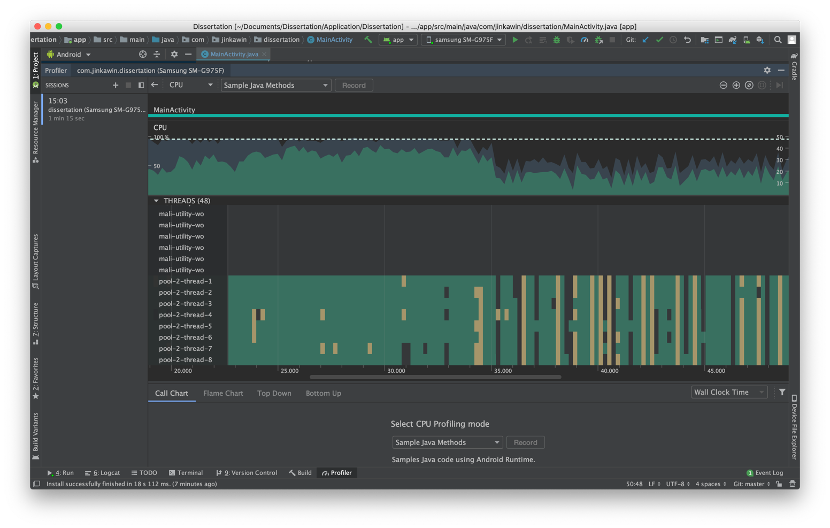
\includegraphics[width=6in]{images/chapter5/YOLO/cpu-usage-8threads.png}
                \caption{CPU Usage of YOLO Model with 8 threads}
                \label{yolo:cpuUsage}
            \end{figure}

            % Memory Usgae
            \begin{figure}[!ht]
                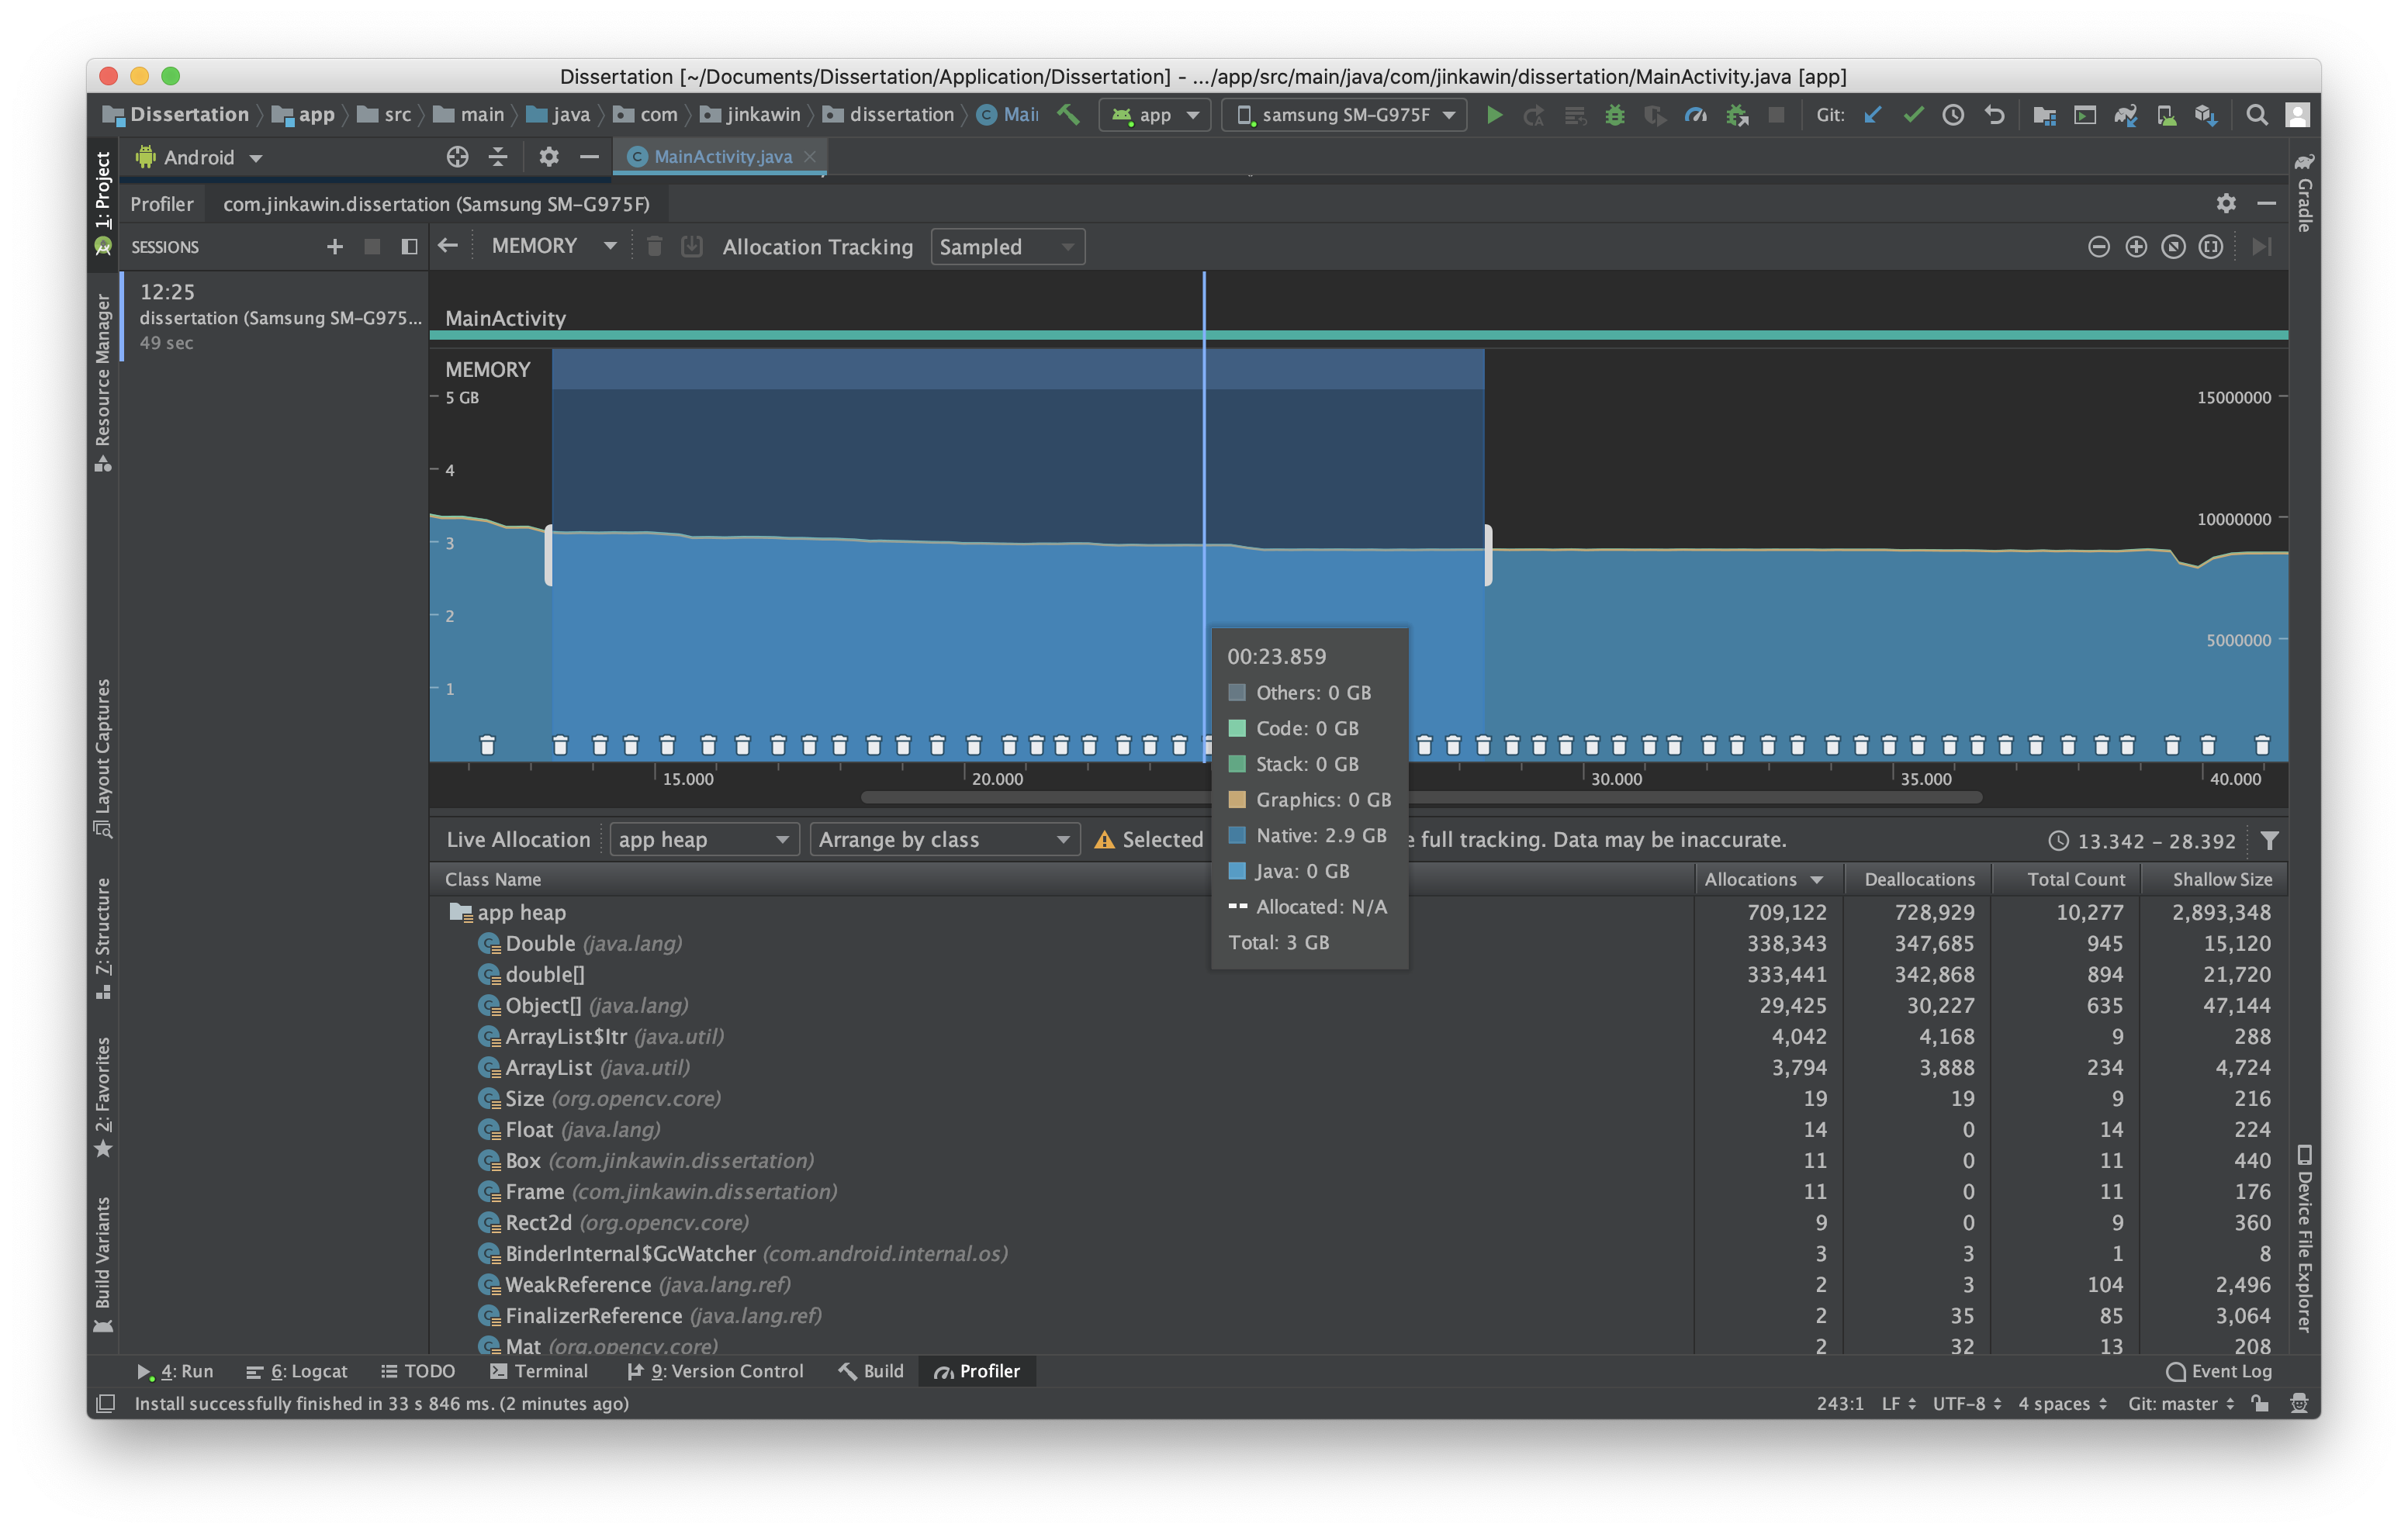
\includegraphics[width=6in]{images/chapter5/gc-problem/gc-collecting.png}
                \caption{Memory Usage of YOLO Model with 8 threads}
                \label{yolo:memoryUsage}
            \end{figure}

            % SSD with multithreading
            For the MobileNet SSD model,
            the calculation time of 2 threads is improved only 16.56 per cent,
            and 8 threads give the best performance with 38.53 per cent as can be seen in table \ref{ssd:official-performace}.
            Objects are not collected by GC in this model, but memory will be freed after processing is finished.
            The improvement computation time of 8 threads by using MobileNet SSD model is better than YOLO model,
            but the speed-up time of both models still lower than an ideal time.

            % Conclusion and tasking about recompile model and NEON
            In summary, the overall performance of YOLO model with multithreading is slightly improved,
            and it becomes worse when using 8 threads.
            Regarding this examination, one of the obvious factors of these problems is
            GC.
            In contrast, the speed-up scale of MobileNet SSD is better than YOLO model because there is no
            GC during processing.
            YOLO model uses more memory than MobileNet SSD in term of variables in double type.

        \subsection{Android Native Development Kit}

            \begin{table}[!htp]\centering
                \scriptsize
                \begin{tabular}{lrrrrrrr}\toprule
                    \multicolumn{2}{c}{Model} &\multicolumn{5}{c}{MobileNet SSD} \\\cmidrule{1-7}
                    \multicolumn{2}{c}{\multirow{2}{*}{}} &\multirow{2}{*}{Sequential Computing} &\multicolumn{4}{c}{Multithreading} \\\cmidrule{4-7}
                    & & &1 Thread &2 Threads &4 Threads &8 Threads \\\midrule
                    \multicolumn{2}{c}{Total Process Time (second)} &6.773 &11.949 &6.597 &6.150 &4.954 \\
                    \multicolumn{2}{c}{Garbage Collector (second)} &- &- &- &- &- \\
                    \multicolumn{2}{c}{Process Time without GC} &- &- &- &- &- \\
                    \multicolumn{2}{c}{Forward Propagation (Total)} &6.659 &- &- &- &- \\
                    \multicolumn{2}{c}{Forward Propagation (Average)} &0.215 &0.382 &0.408 &0.613 &0.970 \\
                    \multicolumn{2}{c}{Forward Propagation (Min)} &0.198 &0.363 &0.394 &0.405 &0.407 \\
                    \multicolumn{2}{c}{Forward Propagation (Max)} &0.236 &0.401 &0.421 &1.043 &2.691 \\
                    \multicolumn{2}{c}{Number of frame} &31 &31 &31 &31 &31 \\
                    \multicolumn{2}{c}{Process per frame (second)} &0.218 &0.385 &0.213 &0.198 &0.160 \\
                    \multicolumn{2}{c}{Improvement} & & &44.79\% &48.53\% &58.54\% \\
                    \bottomrule
                \end{tabular}

                \caption{MobileNet SSD Model with OpenCV official build in C++}\label{ssd:official-performace-cpp}
            \end{table}

            As mentioned in the chapter \ref{implement},
            detection process and distance measurement can be written in C++ to achieve higher performance.
            As it can be seen in table \ref{ssd:official-performace-cpp},
            the performance of using 2 threads is improved 44.79 per cent when compared to using 1 thread,
            and the performance is fastened up to 58.54 per cent when using 8 threads.
            However, there are 2 issues of this implementation.
            The first issues is the forward propagation time.
                Theoretically, the processing time of sequential computing and using a single thread should be the same.
                In contrast, the forward propagation time of single thread was doubled,
                which causes total process time increase.
                Due to the thread management system in C++ is different when compared to Java.
                In C++, the thread is managed by OpenCV's parallelism framework, while
                the thread pool is used in Java which is recommended by Android's document \cite{ANDROID-01}.
            The second issue is the total process time.
                Although writing in C++ is able to achieve theoretical speed-up,
                the overall performance is slightly better when compared to Java.

        \subsection{NEON Instruction}
            OpenCV library provides a shared library, which is officially built by OpenCV.
            However, the library is built to support all CPU chipsets, and many features and conditions were flagged during building.
            The library is needed to be manually built from scratch to evaluate the performance of NEON.
            OpenCV shared library was manually built into two versions: version with NEON and version without NEON.
            To maximise the performance of the NEON version, OpenCV is forced to be built with NEON instruction regardless of any condition,
            and it will support only ARMv8-A 64-bit architecture.

            \begin{table}[!htp]\centering
                \scriptsize
                \begin{tabular}{lrrrrrrr}\toprule
                    \multicolumn{2}{c}{Model} &\multicolumn{5}{c}{MobileNet SSD without NEON} \\\cmidrule{1-7}
                    \multicolumn{2}{c}{\multirow{2}{*}{}} &\multirow{2}{*}{Sequential Computing} &\multicolumn{4}{c}{Parallel Computing} \\\cmidrule{4-7}
                    & & &1 Thread &2 Threads &4 Threads &8 Threads \\\midrule
                    \multicolumn{2}{c}{Total Process Time (second)} &17.308 &19.030 &15.172 &11.797 &10.624 \\
                    \multicolumn{2}{c}{Garbage Collector (second)} &- &- &- &- &- \\
                    \multicolumn{2}{c}{Process Time without GC} &- &- &- &- &- \\
                    \multicolumn{2}{c}{Forward Propagation (Total)} &17.193 &17.848 &- &- &- \\
                    \multicolumn{2}{c}{Forward Propagation (Average)} &0.555 &0.576 &0.926 &1.416 &2.462 \\
                    \multicolumn{2}{c}{Forward Propagation (Min)} &0.519 &0.545 &0.582 &0.756 &1.310 \\
                    \multicolumn{2}{c}{Forward Propagation (Max)} &0.586 &0.654 &1.412 &2.593 &5.308 \\
                    \multicolumn{2}{c}{Number of frame} &31 &31 &31 &31 &31 \\
                    \multicolumn{2}{c}{Process per frame (second)} &0.558 &0.614 &0.489 &0.381 &0.343 \\
                    \multicolumn{2}{c}{Improvement} & & &20.27\% &38.01\% &44.17\% \\
                    \bottomrule
                \end{tabular}

                \caption{MobileNet SSD Model with OpenCV manully build ({\bf without} NEON)}\label{ssd:non-neon-performance}
            \end{table}

            \begin{table}[!htp]\centering
                \scriptsize
                \begin{tabular}{lrrrrrrr}\toprule
                    \multicolumn{2}{c}{Model} &\multicolumn{5}{c}{MobileNet SSD with NEON} \\\cmidrule{1-7}
                    \multicolumn{2}{c}{\multirow{2}{*}{}} &\multirow{2}{*}{Sequential Computing} &\multicolumn{4}{c}{Multithreading} \\\cmidrule{4-7}
                    & & &1 Thread &2 Threads &4 Threads &8 Threads \\\midrule
                    \multicolumn{2}{c}{Total Process Time (second)} &4.006 &6.079 &4.208 &3.127 &2.890 \\
                    \multicolumn{2}{c}{Garbage Collector (second)} &- &- &- &- &- \\
                    \multicolumn{2}{c}{Process Time without GC} &- &- &- &- &- \\
                    \multicolumn{2}{c}{Forward Propagation (Total)} &3.927 &4.950 &- &- &- \\
                    \multicolumn{2}{c}{Forward Propagation (Average)} &0.126 &0.159 &0.225 &0.339 &0.645 \\
                    \multicolumn{2}{c}{Forward Propagation (Min)} &0.117 &0.128 &0.131 &0.190 &0.266 \\
                    \multicolumn{2}{c}{Forward Propagation (Max)} &0.135 &0.250 &0.295 &0.596 &1.798 \\
                    \multicolumn{2}{c}{Number of frame} &31 &31 &31 &31 &31 \\
                    \multicolumn{2}{c}{Process per frame (second)} &0.129 &0.196 &0.136 &0.101 &0.093 \\
                    \multicolumn{2}{c}{Improvement} & & &30.78\% &48.56\% &52.46\% \\
                    \bottomrule
                \end{tabular}

                \caption{Video Processing with MobileNet SSD Model ({\bf with} NEON)}\label{ssd:neon-performance}
            \end{table}

            After OpenCV library is manually built and forced to be compiled with NEON instruction,
            the performance of human detection is significantly improved.
            As can be seen in table \ref{ssd:non-neon-performance} and \ref{ssd:neon-performance},
            the sequential computing took 4 second for processing human detection,
            which is faster than OpenCV without NEON 76.85 percent.
            In addition, multithreading can process 31 frames of the video up to 2.890 seconds,
            which is faster than OpenCV without NEON 72.79 per cent and OpenCV official build 42.93 per cent.
            For this performance, video can be processed 10.75 frames per second.
            In addition, according to rendering technique in chapter \ref{implement},
            a real-time video from the camera can display up to 25 frames per second.

    % Analyse
    Thus far, these results were not achieved theoretical,
    and this application did not achieve processing and displaying 30 FPS even if
    multithreading and NEON are implemented.
    This underachieved performance could be caused by mulithreading itself.
    A forward propagation time, which took most of the computation time, is doubled when the number of threads is increased.
        One of the issues that emerge from this finding is parallelisation in the OpenCV library.
        Some function underneath the forward propagation function is parallelised by using multithreading.
        Then, when a frame processing thread is created, a number of threads may exceed the number of physical cores.
        Thus, threads are interrupted, and it caused a context switching overhead.
    Besides, the calculation time of using a single thread is always greater than
    the calculation time un sequential computing and it could be caused by this problem.

%%%%%%%%%%%%%%%%%%%%%%%%%%%%%%%%%%%%%%%%%%%%%%%%%%%%%%%%%%%%%%%%%%%
\chapter{Conclusion}\label{conclusion}

    This project was undertaken to build a social distancing detection application on the Android operating system,
    and to maximise detection performance by using various technologies and techniques.

    % What I have achieved
    The results of this implementation show that the combination of the MobileNet SSD model,
    manually built OpenCV with NEON, and using 8 threads provides the best performance \cite{tensorflow2015-whitepaper}, \cite{opencv_library}, \cite{NEON-ARM}.
    The computation time of a pre-recorded single frame took 93 milliseconds or 10.752 frames per second,
    and this application can display 25 frames of video in 1 second on a live camera
    with the help of rendering technique.
    The accuracy of the YOLO model was higher than MobileNet SSD model.
    However, computational time and memory usage of the YOLO model was worse than MobileNet SSD.
    The YOLO model computation time of 31 frames by using 8 threads was 99.441 seconds,
    while the MobileNet SSD model took 5.064 seconds.
    In addition, if NEON is implemented the MobileNet SSD mobile is able to process 31 frames in 2.890 seconds.

    \section{Limitation}
        Limitations of this application have been found during development.
        There are 3 main limitations of this application.
        The first limitation is processing with a graphics processing unit (GPU).
            Due to OpenCV, currently, supports 3 GPUs which are Intel, Nvidia, and AMD.
            However, the testing environment, Samsung Galaxy S10+, has an ARM Mali GPU.
        Secondly, processing video in real-time with the YOLO model cannot be achieved.
            YOLO model requires a great amount of resources including computing power and memory.
            Because of limited memory and high demand of memory, garbage collector causes interruptions and frozes the application.
            In addition, using only CPU cannot achieve an ideal processing time even though multithreading is applied.
            However, the YOLO model is able to detect human more efficiently than the MobileNet SSD.
            Thus, there is a tread-off between processing time and accuracy.
            Finally, the resolution of the video is limited.
            Regarding performance, the proposed application processes video in low resolution,
            which is 540x480 pixels.
            Processing high-resolution video needs more computing power and resources to process in real-time,
            which are limited in mobile phones.

    \section{Future Work}
    Considering the studies and limitation of this project,
    there are many possible aspects that can be done for further development.

    The first aspect that may improve the performance is using GPUs.
        According to the findings, these show that the performance cannot be enhanced further by using CPU with OpenCV library.
        The more accuracy and performance, the more computing power is needed.
        Using GPUs to compute forward propagation may significantly reduce the processing time.
        To support using GPUs, the library must be changed from OpenCV to others that support
        GPU implementation, such as TensorFlow \cite{tensorflow2015-whitepaper}.
        Also, OpenCL can be used with TensorFlow to do parallelisation.
        These can be implemented in Native code to maximise the performance
        and may achieve higher accuracy, FPS, and resolution.

    The second aspect is implementing single instruction, multiple data (SIMD) in other modules,
        which may gain processing performance.
        There are parts of the implementation and function that are written in Java, and these do not support SIMD.
        To maximise the performance, rewriting the programme in C or C++ with SIMD is needed.
        For instance, calculating the distance between detected humans is written in Java,
        so this function can be rewritten in C++ to support SIMD.
        In addition, implementing SIMD can be done in other environments for comparing performance and gaining insight.
        For example, Streaming SIMD Extensions (SSE) can be implemented on Intel's processor and AMD's processor to improve the performance \cite{intel-sse}.
        Besides, processing on Intel's processor can be optimised by using the Math Kernel Library (MKL) \cite{intel-alt}.
        Implementing SIMD and evaluating other environments may gain an understanding of limitation and overhead of computation by using CPU.

    Finally, another aspect is improving the usability of the application.
        Features can be added to the application to improve practical usability.
        For instance, face mask detection can be implemented into the application \cite{facemask-detection},
        and the performance can be enhanced by using multithreading and SIMD.
        In addition, this application can be integrated with other systems
        for practical usage such as a security system.


\appendix % first appendix
%%%%%%%%%%%%%%%%%%%%%%%%%%%%%%%%%%%%%%%%%%%%%%%%%%%%%%%%%%%%%%%%%%%
\chapter{Existing Applications}\label{intro}

    \begin{figure}[!ht]
        \centering
        \begin{minipage}{.5\textwidth}
            \centering
            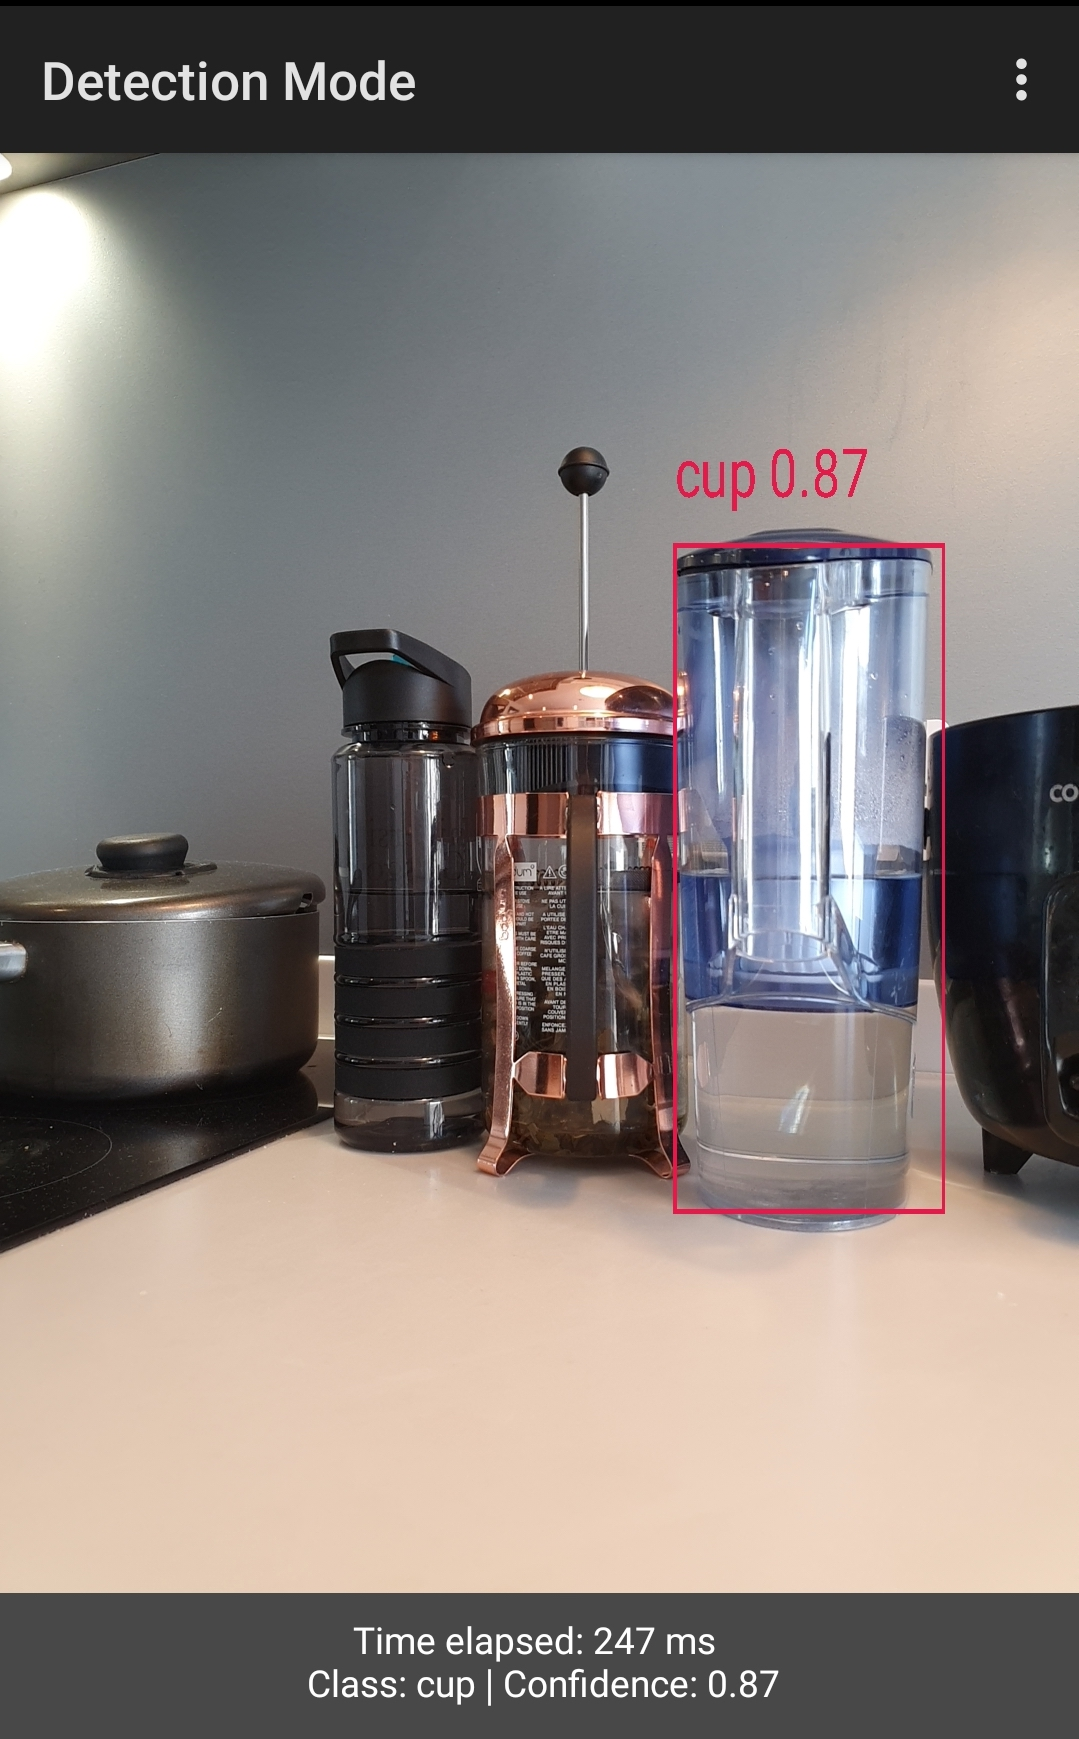
\includegraphics[width=2in]{images/chapter2/object-detector.jpg}
            \captionof{figure}{Object Detector}
            \label{appendix:obj-detector}
        \end{minipage}%
        \begin{minipage}{.5\textwidth}
            \centering
            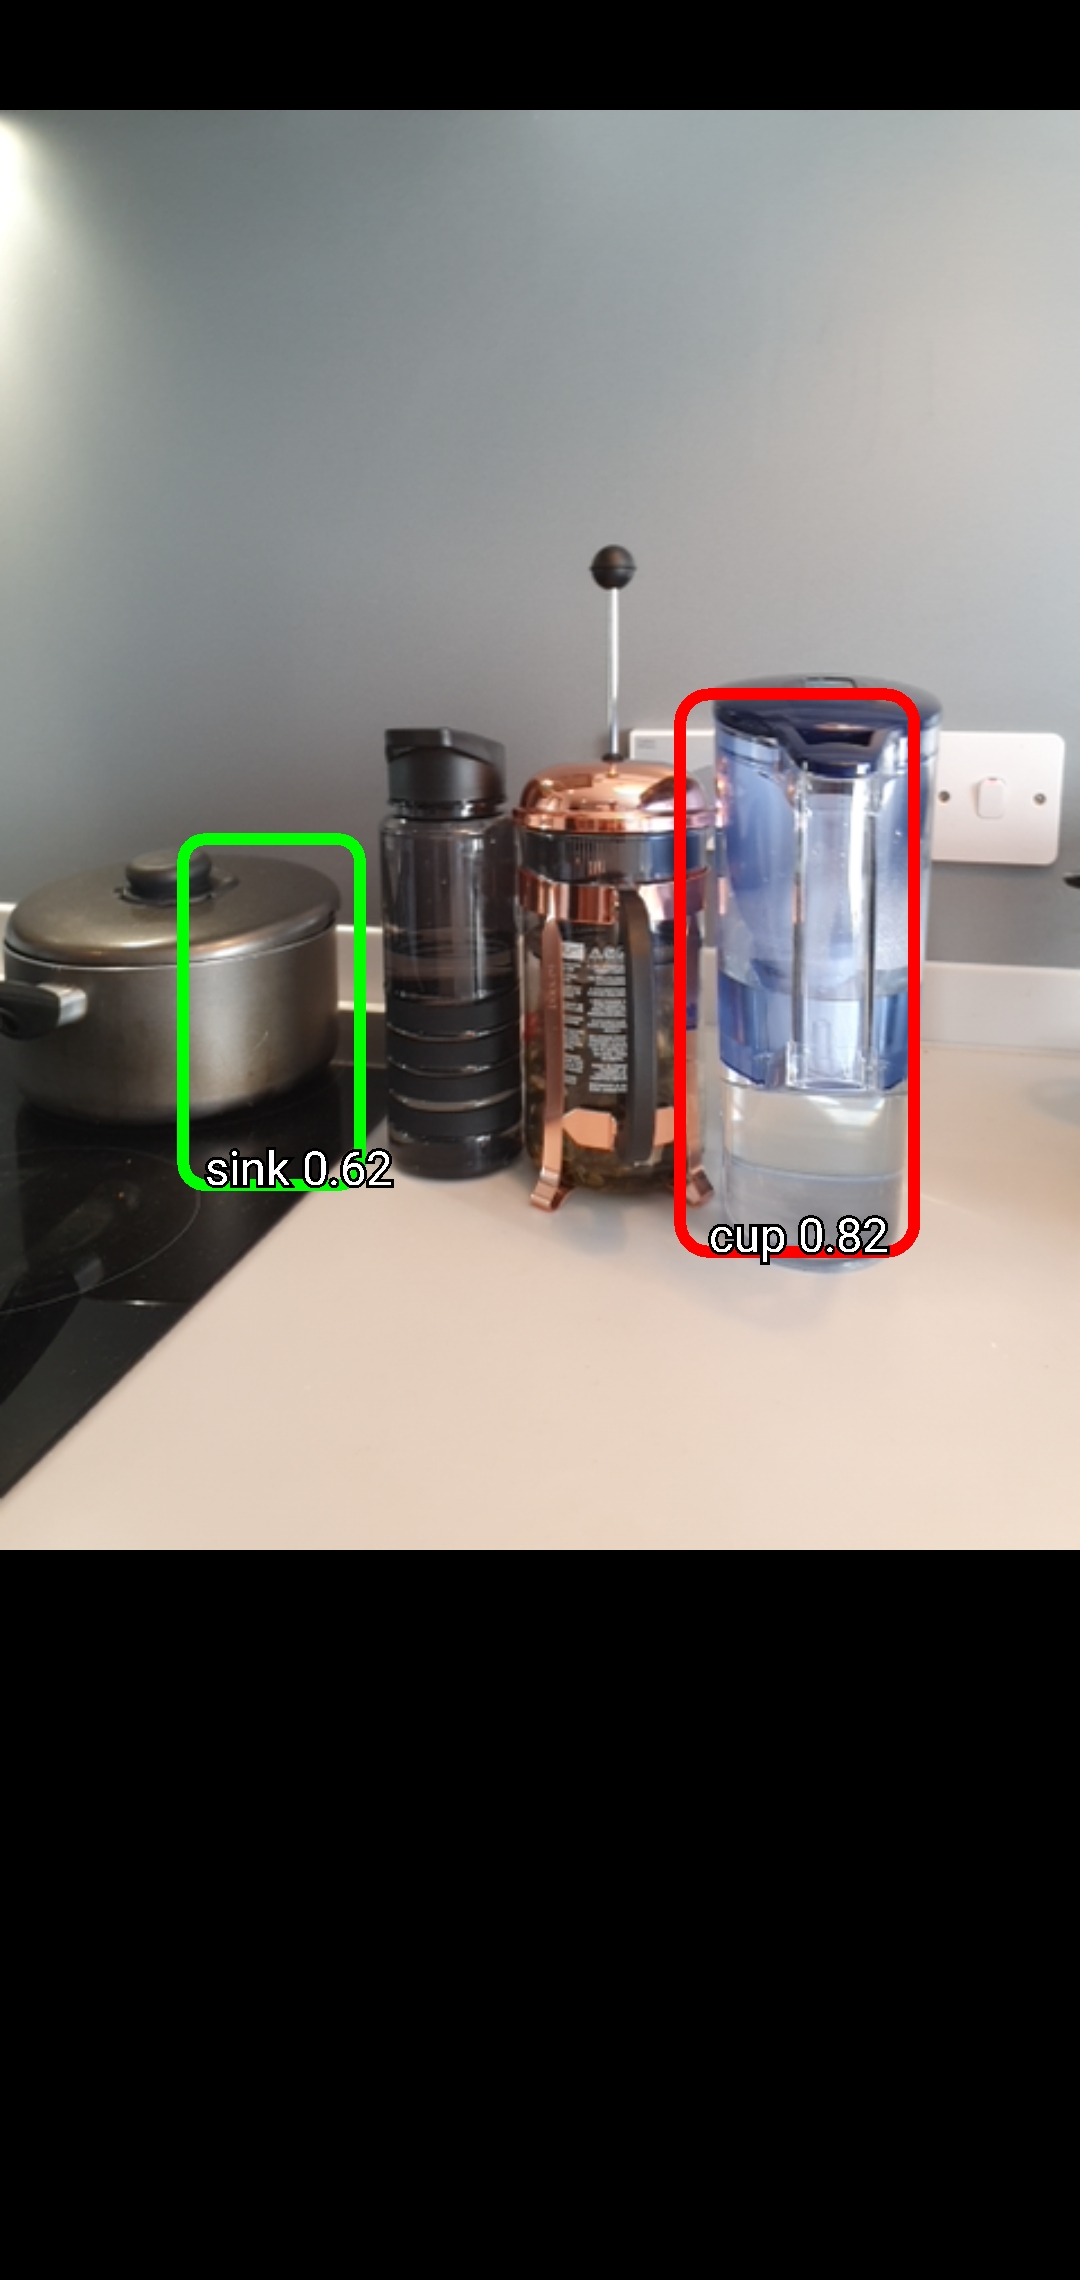
\includegraphics[width=2in]{images/chapter2/ml-detection-tf.jpg}
            \captionof{figure}{TensorFlow Object Detection}
            \label{appendix:ts-obj-detection}
        \end{minipage}
    \end{figure}

    \begin{figure}[!ht]
        \centering
        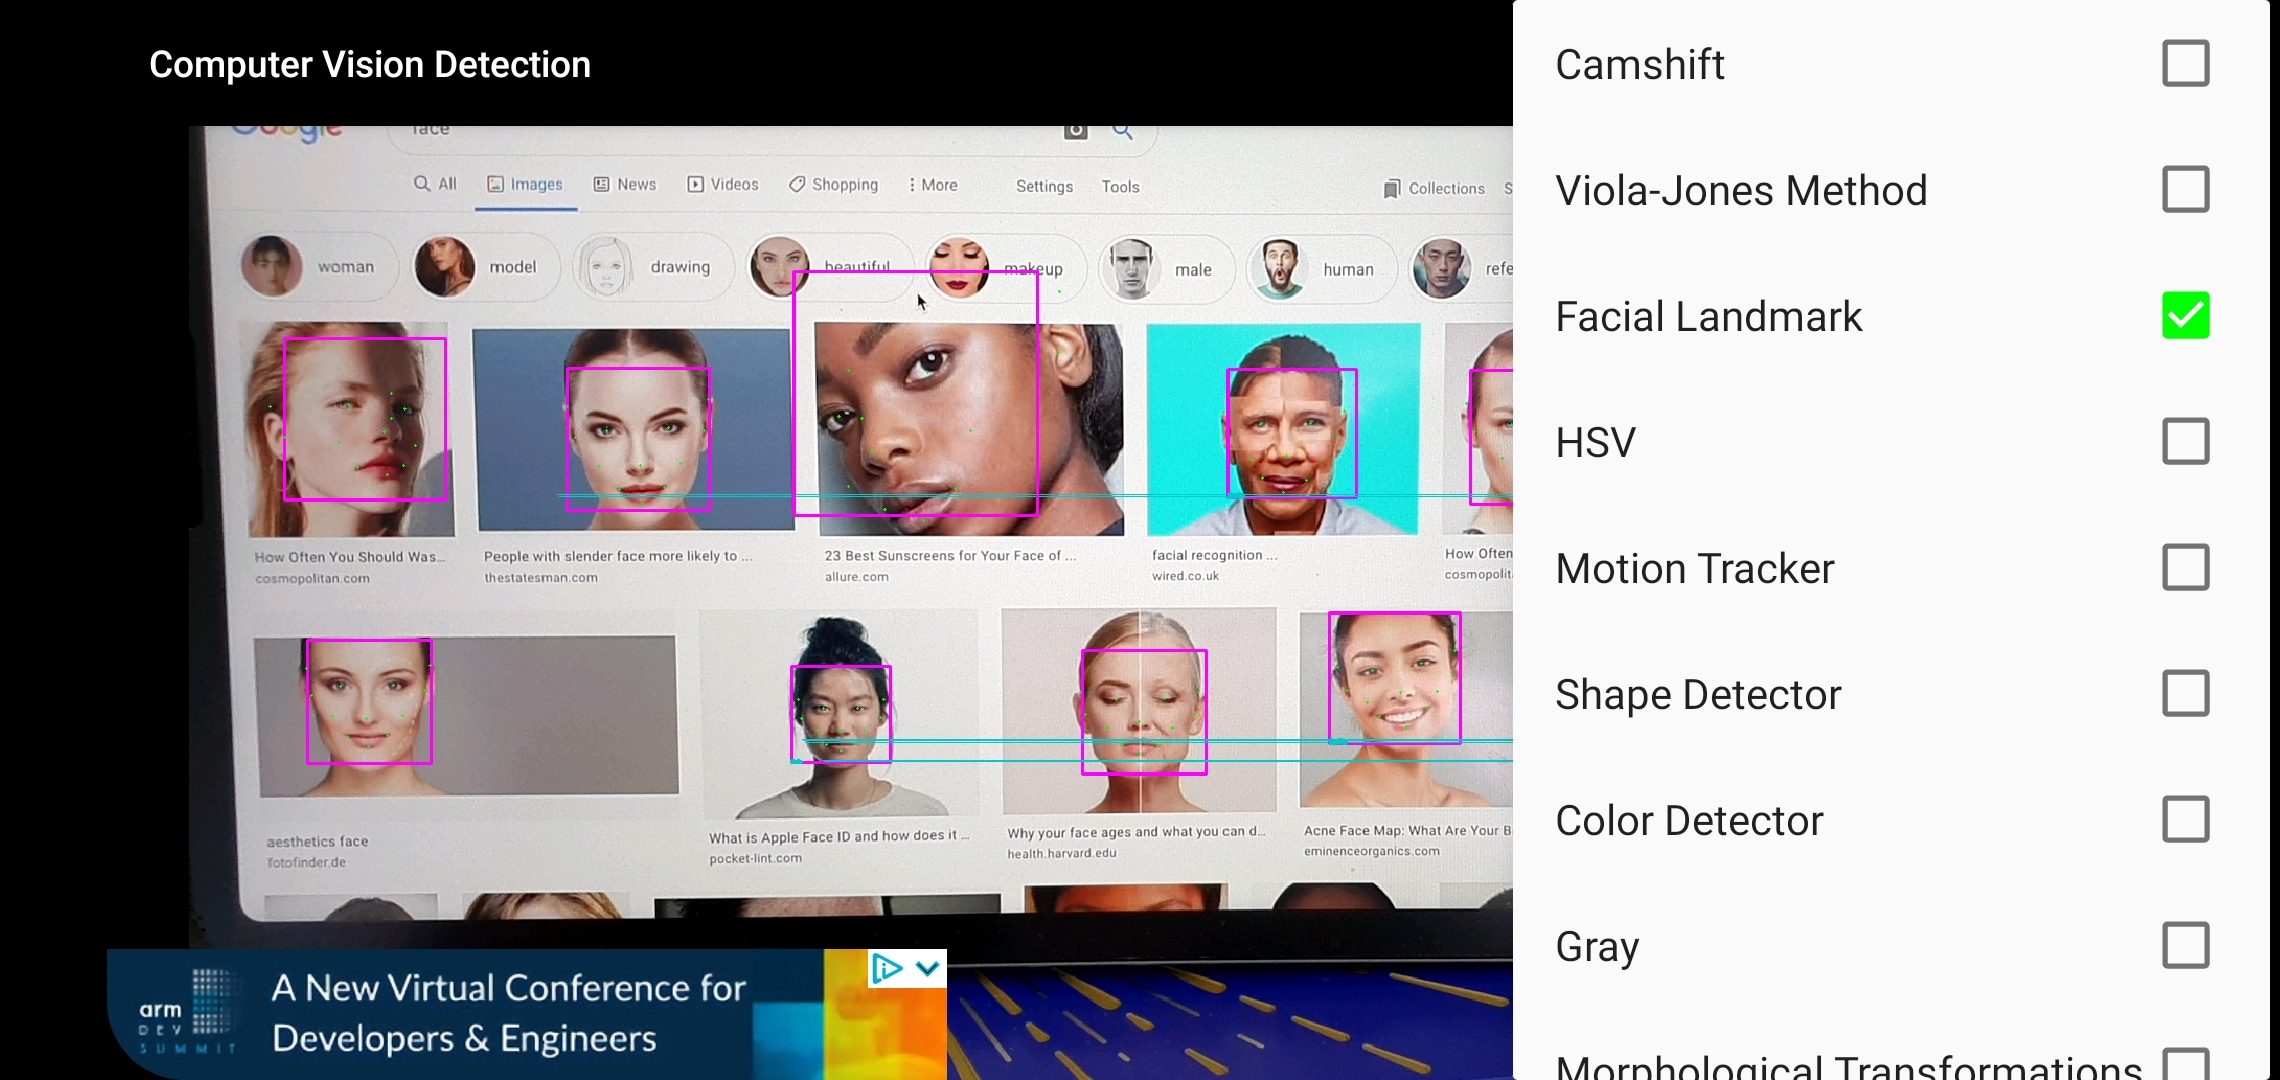
\includegraphics[width=3in]{images/chapter2/cv-detection.jpg}
        \caption{Computer Vision Detection}
        \label{appendix:cv-detection}
    \end{figure}

%%%%%%%%%%%%%%%%%%%%%%%%%%%%%%%%%%%%%%%%%%%%%%%%%%%%%%%%%%%%%%%%%%%
\chapter{Application Screenshot}\label{intro}

    \begin{figure}[h!]
        \centering
        \begin{subfigure}{.5\textwidth}
        \centering
        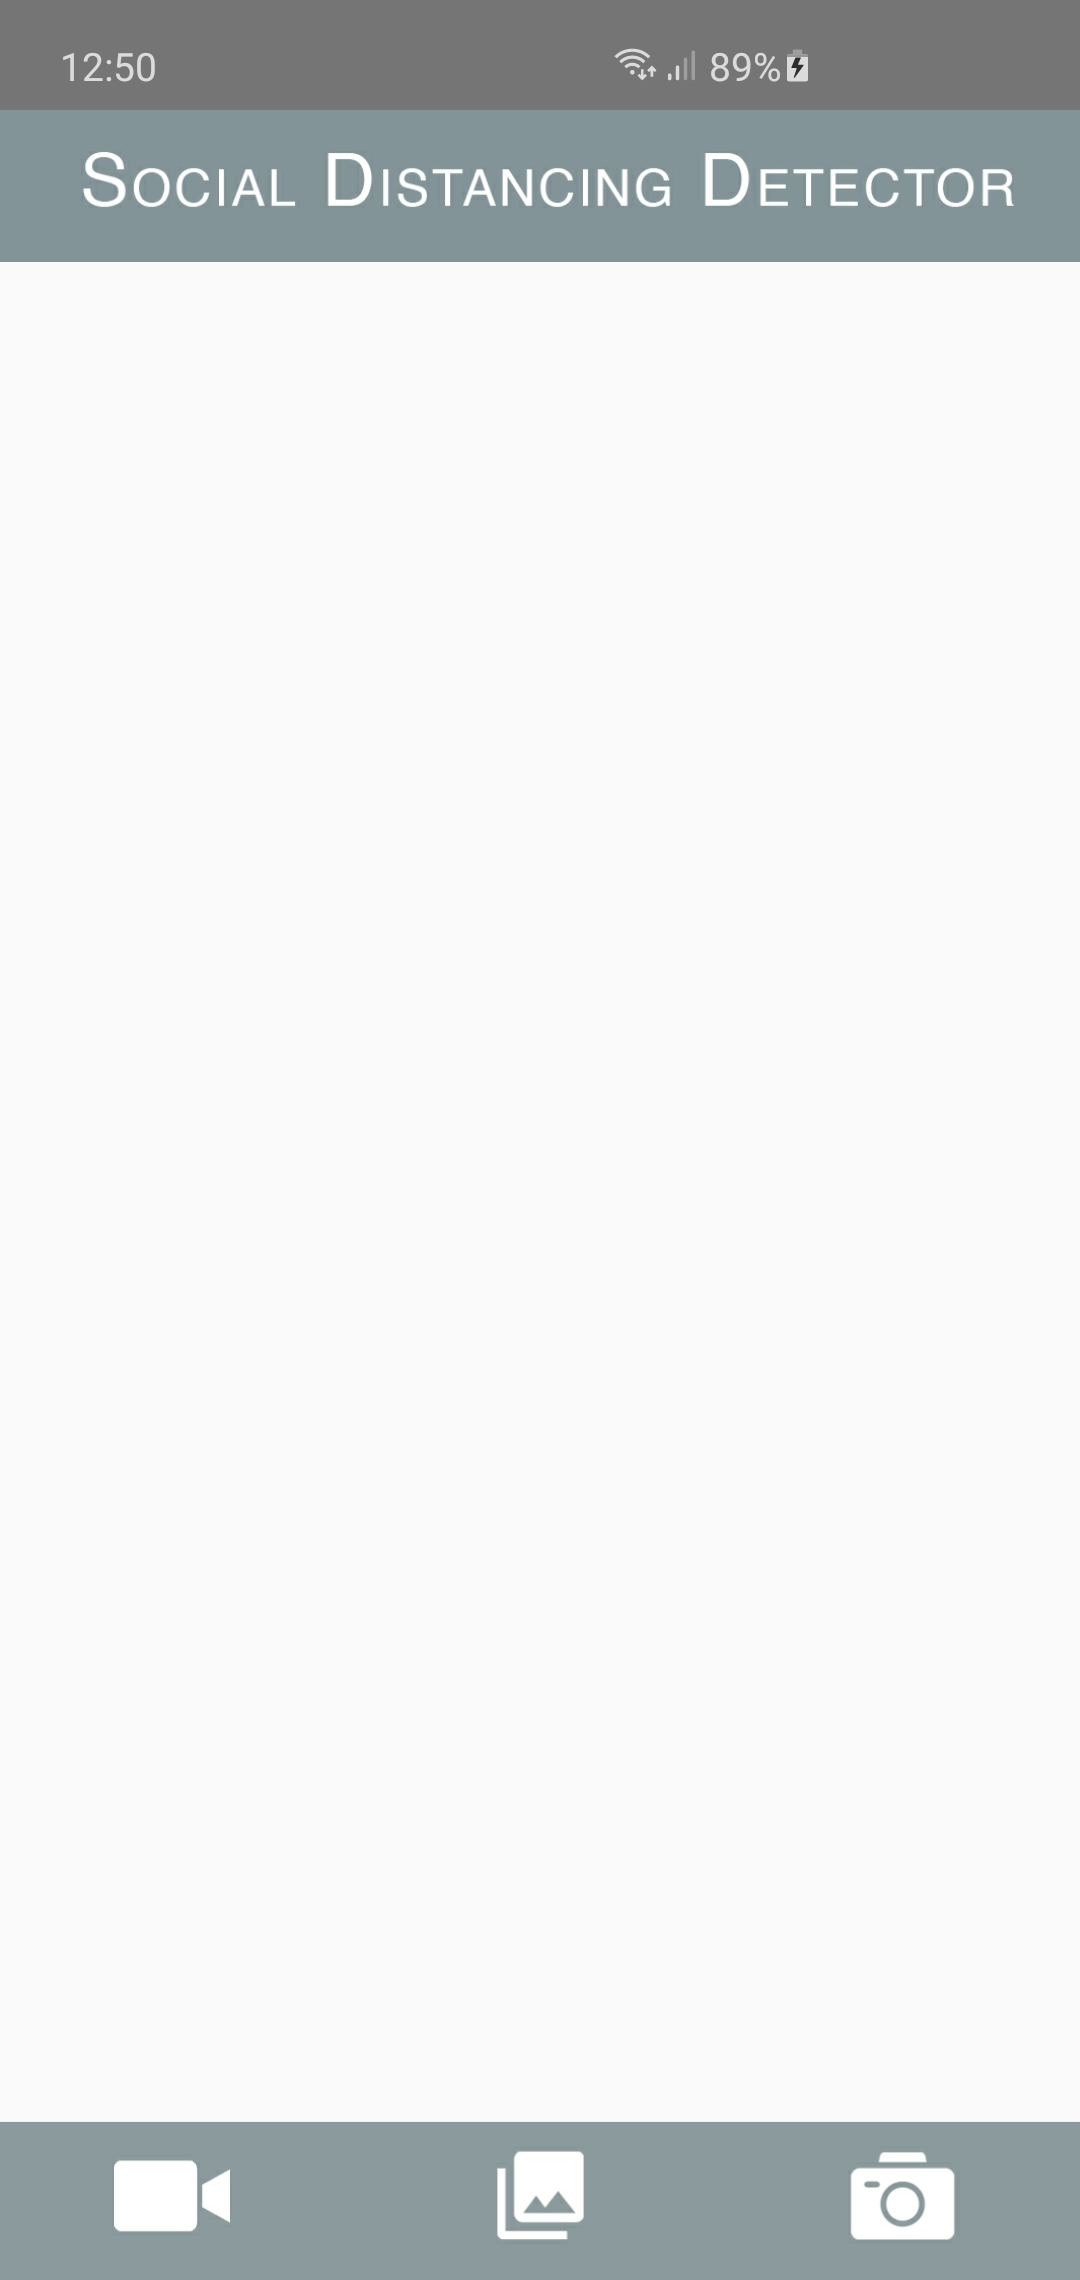
\includegraphics[width=3in]{images/appendix-b/sh-main.jpg}
        \caption{Main Menu}
        \label{appendix-b:mainMenu}
        \end{subfigure}%
        \begin{subfigure}{.5\textwidth}
        \centering
        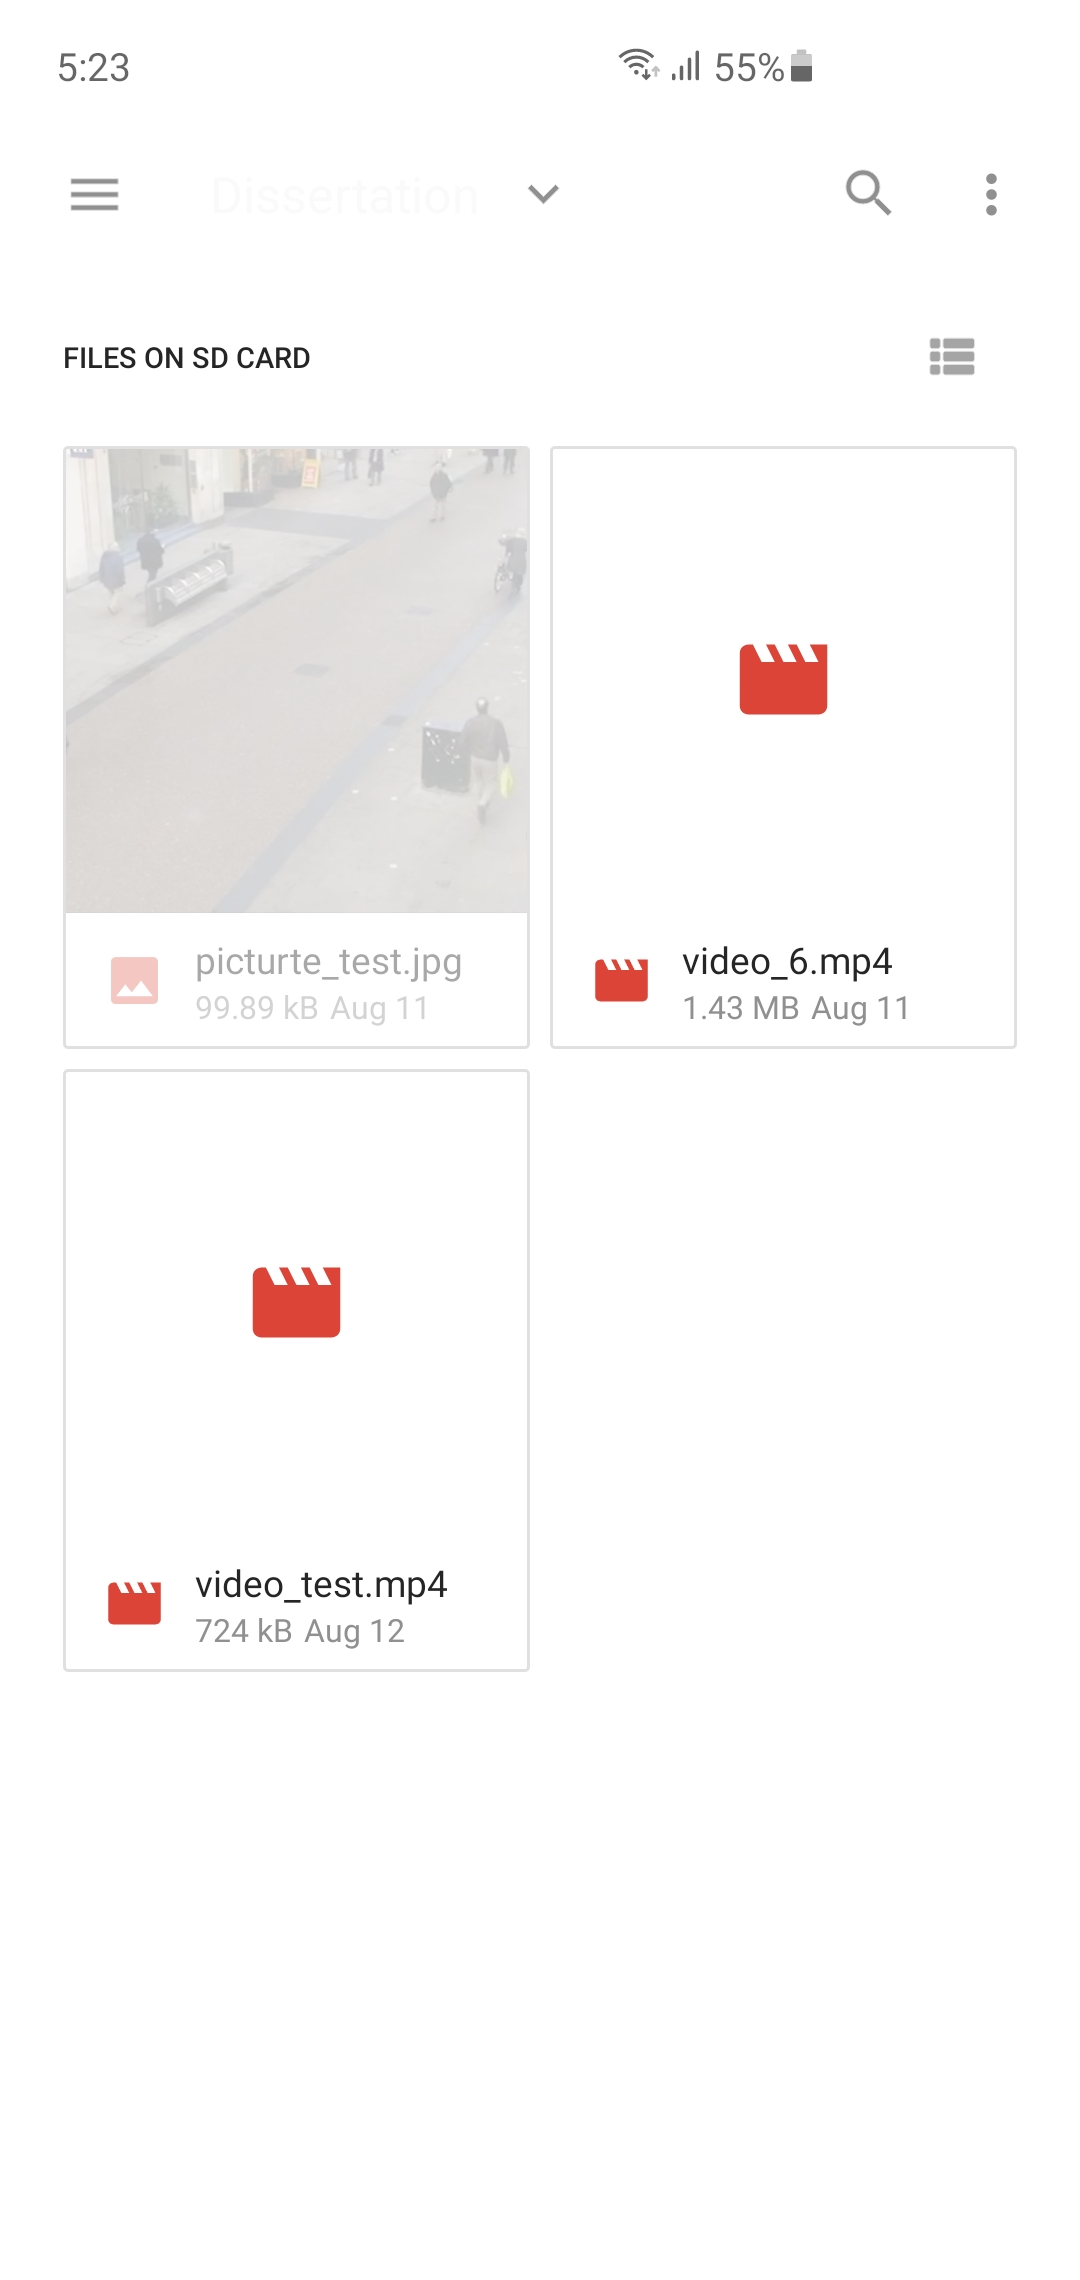
\includegraphics[width=3in]{images/appendix-b/sh-choosing.jpg}
        \caption{Choosing Existing File from Gallery}
        \label{appendix-b:filePicker}
        \end{subfigure}
        \caption{Application Interface}
        \label{appendix-b:process}
    \end{figure}

    \begin{figure}[h!]
        \centering
        \begin{subfigure}{.5\textwidth}
        \centering
        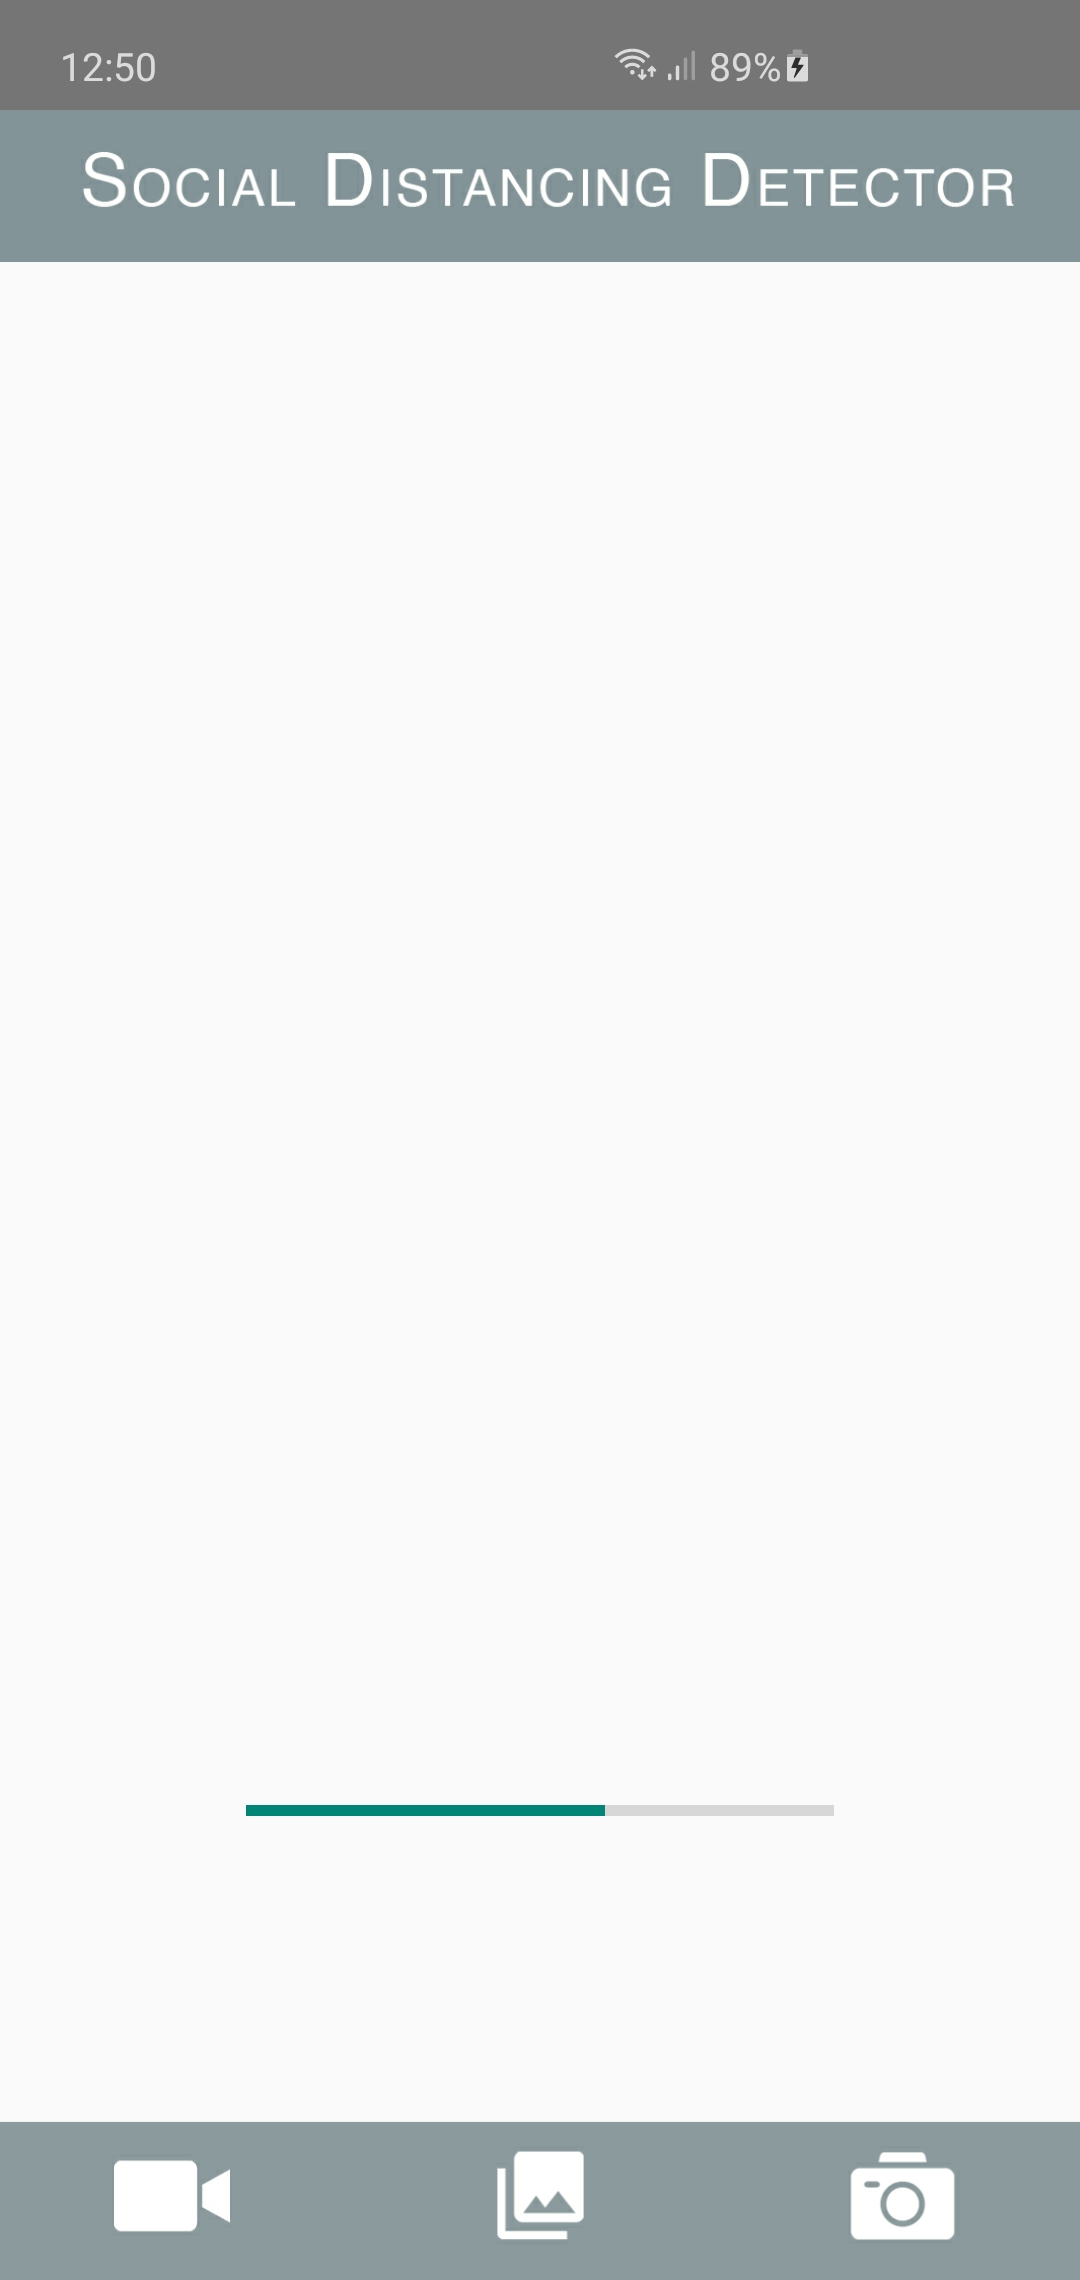
\includegraphics[width=3in]{images/appendix-b/sh-processing.jpg}
        \caption{Status Bar While Processing}
        \label{appendix-b:statusBar}
        \end{subfigure}%
        \begin{subfigure}{.5\textwidth}
        \centering
        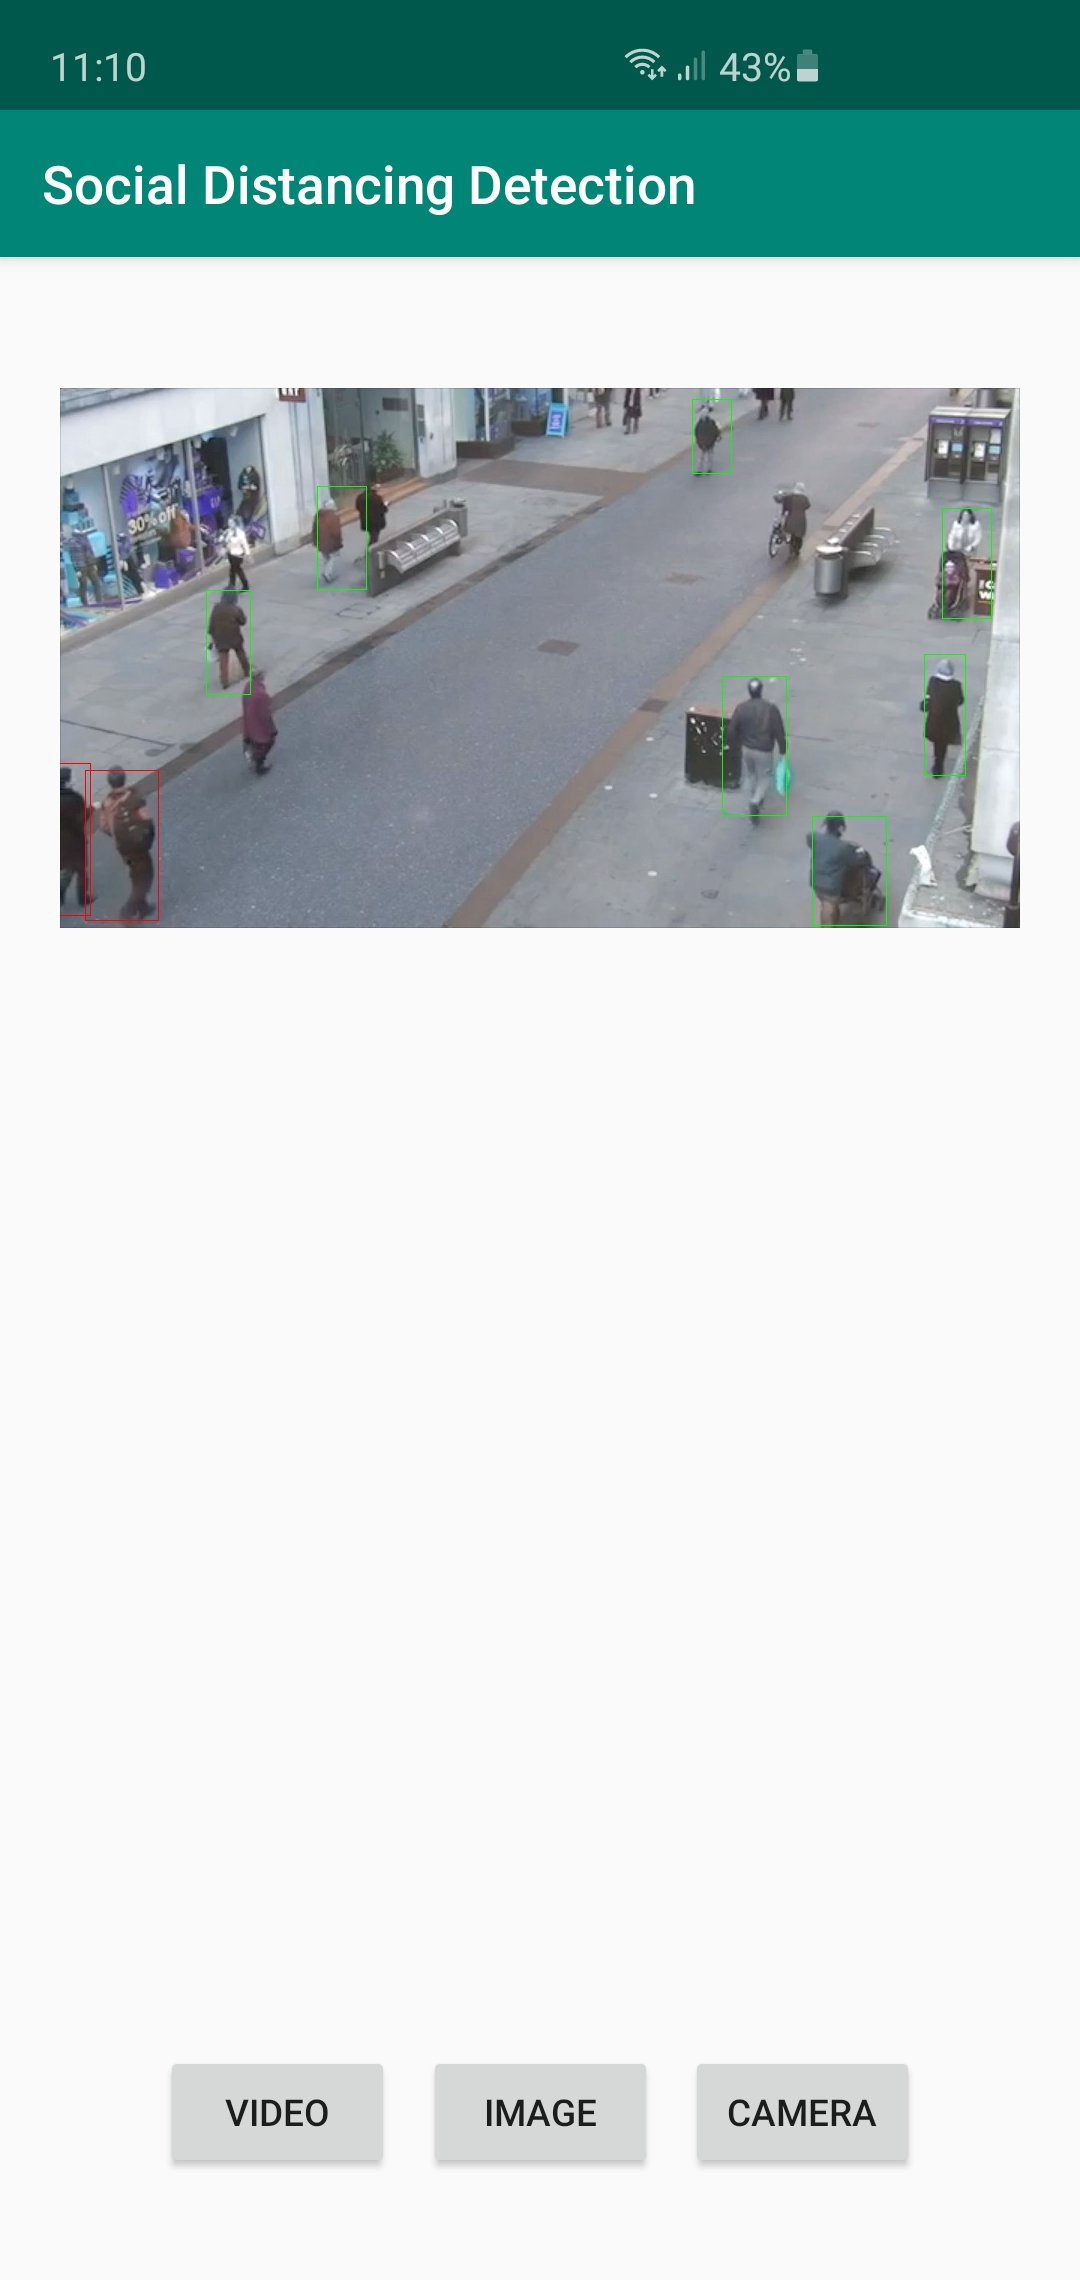
\includegraphics[width=3in]{images/appendix-b/sh-output.jpg}
        \caption{Display a proessed image or video}
        \label{appendix-b:result}
        \end{subfigure}
        \caption{Processing pre-recorded file}
        \label{appendix-b:process}
    \end{figure}

    \begin{figure}[!ht]
        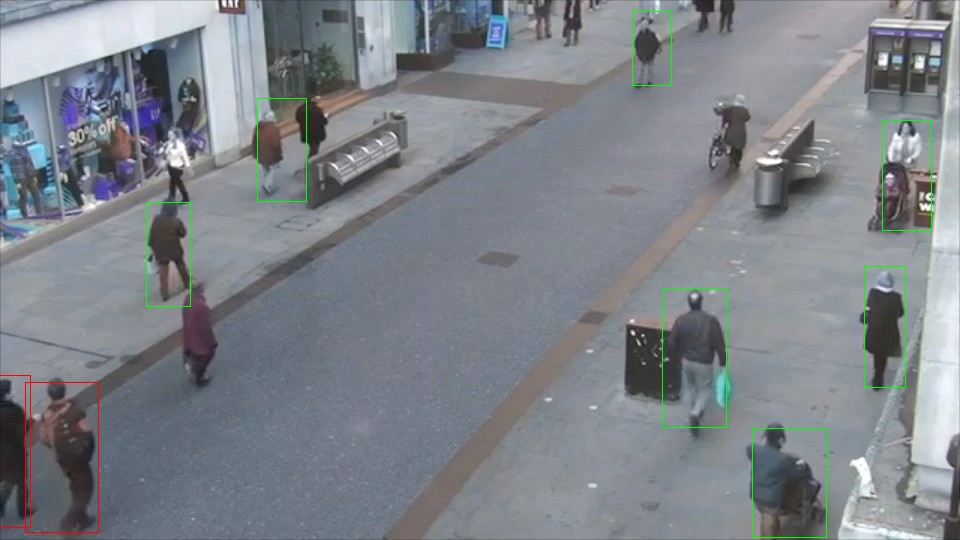
\includegraphics[width=6in]{images/chapter5/application/picture-detection.jpg}
        \caption{Social Distancing Detection from Picture}
        \label{appendix-b:sampleResult}
    \end{figure}

    \begin{figure}[!ht]
        \centering
        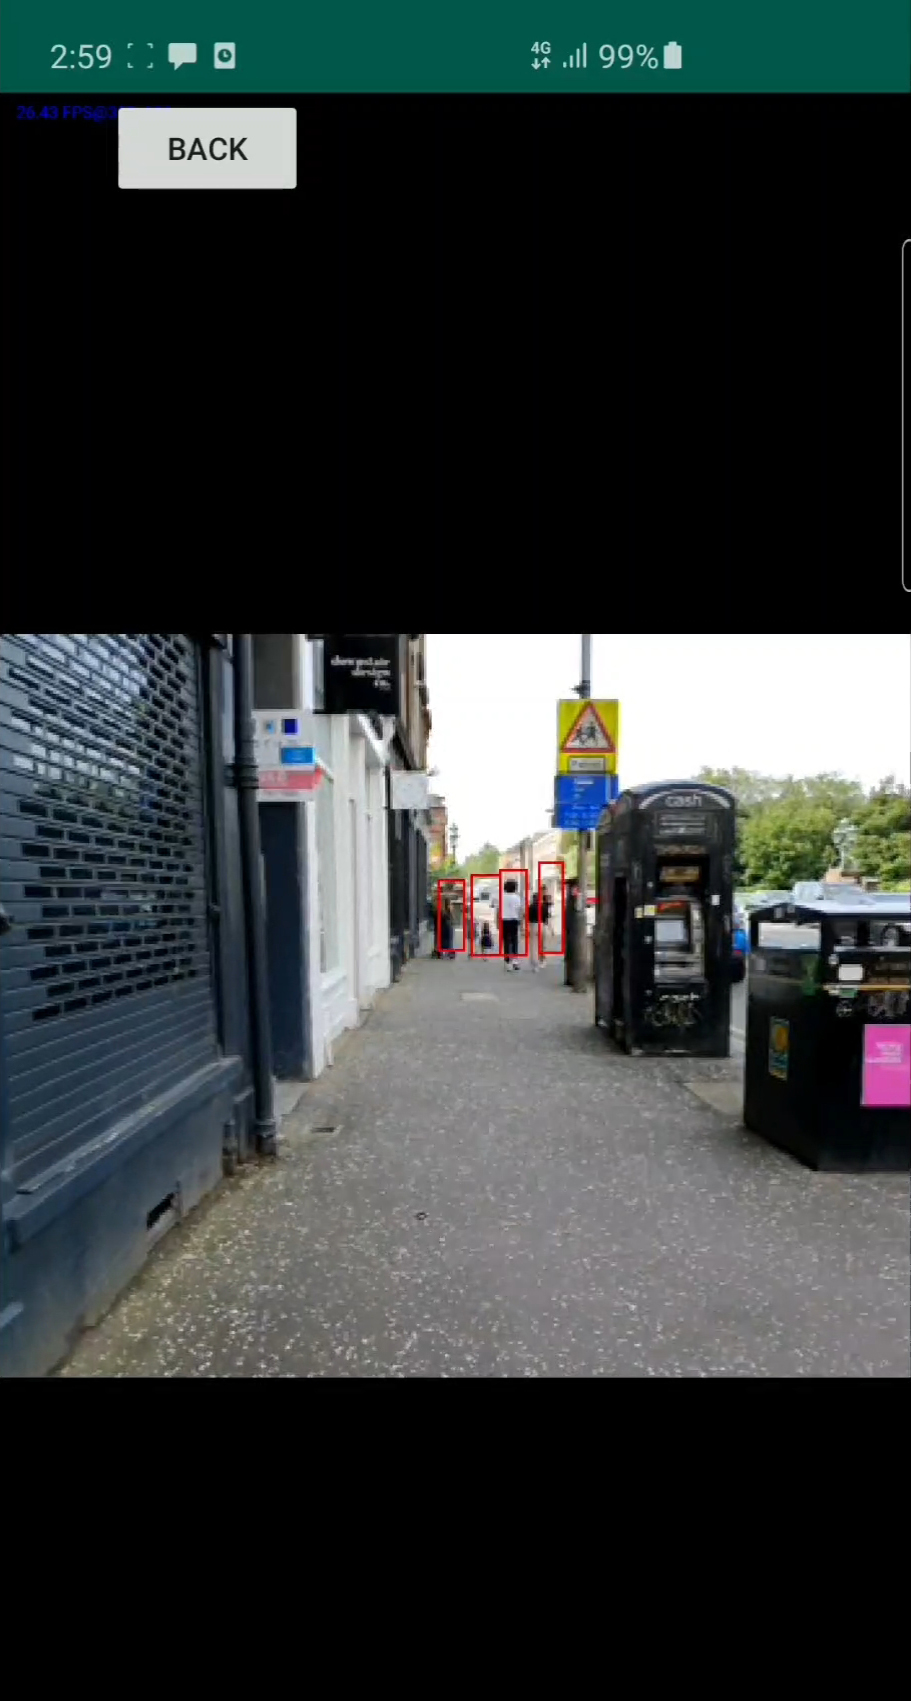
\includegraphics[width=3in]{images/chapter5/application/camera-detection.jpg}
        \caption{Social Distancing Detection by Using Camera}
        \label{appendix-b:camera}
    \end{figure}

%%%%%%%%%%%%%%%%%%%%%%%%%%%%%%%%%%%%%%%%%%%%%%%%%%%%%%%%%%%%%%%%%%%
% it is fine to change the bibliography style if you want
\bibliographystyle{plain}
\bibliography{mproj}
\end{document}
